%% LyX 1.6.0svn created this file.  For more info, see http://www.lyx.org/.
%% Do not edit unless you really know what you are doing.
\documentclass[english]{article}
\usepackage[T1]{fontenc}
\usepackage[latin9]{inputenc}
\setlength{\parskip}{\medskipamount}
\setlength{\parindent}{0pt}
\usepackage{url}
\usepackage{amsmath}
\usepackage{graphicx}
\usepackage{amssymb}
\usepackage{babel}
\usepackage[unicode=true, pdfusetitle,
 bookmarks=true,bookmarksnumbered=false,bookmarksopen=false,
 breaklinks=false,pdfborder={0 0 1},backref=false,pagebackref=false,
 colorlinks=false]
 {hyperref}


%%%%%%%%%%%%%%%%%%%%%%%%%%%%%% LyX specific LaTeX commands.
%% Because html converters don't know tabularnewline
\providecommand{\tabularnewline}{\\}

%%%%%%%%%%%%%%%%%%%%%%%%%%%%%% Textclass specific LaTeX commands.
\usepackage{Sweave}
\newcommand{\Rcode}[1]{{\texttt{#1}}}
\newcommand{\Robject}[1]{{\texttt{#1}}}
\newcommand{\Rcommand}[1]{{\texttt{#1}}}
\newcommand{\Rfunction}[1]{{\texttt{#1}}}
\newcommand{\Rfunarg}[1]{{\textit{#1}}}
\newcommand{\Rpackage}[1]{{\textit{#1}}}
\newcommand{\Rmethod}[1]{{\textit{#1}}}
\newcommand{\Rclass}[1]{{\textit{#1}}}

%%%%%%%%%%%%%%%%%%%%%%%%%%%%%% User specified LaTeX commands.
% Meta information - fill between {} and do not remove %
% \VignetteIndexEntry{Factor Analysis in R}
% \VignetteDepends{FAiR}
% \VignetteKeywords{models, multivariate}
% \VignettePackage{FAiR}
\usepackage{fullpage}
\usepackage{times}

\begin{document}

\title{FA$i$R Vignette}


\author{Ben Goodrich}

\maketitle
\textbf{This vignette is intended to be a quick reference that defines
terms and illustrates how to use the pop-up menus. Large parts will
not make a great deal of sense outside the introduction to SEFA and
lexical optimization in Goodrich (2008a) and Goodrich (2008b).}

\tableofcontents{}

\newpage{}


\section{Notation}

Some notation is provided so that the reader can refer back to it.
For simplicity, I usually do not distinguish the notation for a population
parameter from the notation for an estimate of that population parameter
here. In particular, note that all models currently in FA$i$R utilize
an {}``embedded correlation'' parameterization.
\begin{itemize}
\item $n$ is the number of outcome variables, which are indexed by $j$
\item $\boldsymbol{\Sigma}$ is the $n\times n$ covariance matrix among
outcomes in the population
\item $\mathbf{S}$ is the $n\times n$ covariance matrix among outcomes
in the sample
\item $\mathbf{s}=\textrm{vecs}\left(\mathbf{S}\right)$ stacks the elements
below and including the diagonal of $\mathbf{S}$ into a vector of
length $n^{\ast}=0.5n\left(n+1\right)$
\item $\boldsymbol{\Gamma}=\textrm{acov}\left(\mathbf{s}\right)$ is the
asymptotic covariance of $\mathbf{s}$ 
\item $r$ is the number of factors, which are indexed by $p$
\item $\boldsymbol{\beta}$ is the $n\times r$ primary pattern matrix with
one column for each factor
\item $\boldsymbol{\Phi}$ is the $r\times r$ correlation matrix among
primary factors
\item $\boldsymbol{\Lambda}$ is used to indicate the primary pattern matrix
only if $\boldsymbol{\Phi}=\mathbf{I}_{r}$
\item $\mathbf{R}^{\ast}=\boldsymbol{\beta}\boldsymbol{\Phi}\boldsymbol{\beta}^{\prime}$
is the reduced correlation matrix with communalities along the diagonal,
denoted by $h_{j}^{2}=R_{jj}^{\ast}$
\item $\boldsymbol{\Theta}^{2}$ is the $n\times n$ diagonal (for now)
covariance matrix among unique factors such that $\Theta_{jj}^{2}=1-h_{j}^{2}$
\item $\mathbf{R}=\mathbf{R}^{\ast}+\boldsymbol{\Theta}^{2}=\boldsymbol{\beta}\boldsymbol{\Phi}\boldsymbol{\beta}^{\prime}+\boldsymbol{\Theta}^{2}$
is the $n\times n$ reproduced correlation matrix with ones along
the diagonal
\item $\boldsymbol{\Omega}$ is the $n\times n$ diagonal matrix of standard
deviations of the manifest variables to be estimated generally
\item $\mathbf{C}=\boldsymbol{\Omega}\mathbf{R}\boldsymbol{\Omega}=\boldsymbol{\Omega}\left(\boldsymbol{\beta\Phi\beta}^{\prime}+\boldsymbol{\Theta}^{2}\right)\boldsymbol{\Omega}$
is the $n\times n$ reproduced covariance matrix and also the expectation
of $\mathbf{S}$
\item $\mathbf{c}=\textrm{vecs}\left(\mathbf{C}\right)$ stacks the elements
below and including the diagonal of $\mathbf{C}$ into a vector of
length $n^{\ast}$
\item $\boldsymbol{\Pi}=\boldsymbol{\beta\boldsymbol{\Phi}}$ is the $n\times r$
primary structure matrix of correlations between outcome variables
and factors
\item $\boldsymbol{\Game}=\boldsymbol{\beta}\times\boldsymbol{\Pi}$ is
the $n\times r$ factor contribution matrix, where $\times$ indicates
element-by-element multiplication
\item $\mathbf{D}=\left[\textrm{Diag}\left(\boldsymbol{\Phi}^{-1}\right)\right]^{-\frac{1}{2}}$
is the $r\times r$ correlation matrix between primary and reference
factors
\item $\boldsymbol{\Psi}=\mathbf{D}\boldsymbol{\Phi}^{-1}\mathbf{D}$ is
the $r\times r$ correlation matrix among reference factors
\item $\boldsymbol{\Upsilon}=\boldsymbol{\beta}\mathbf{D}$ is the $n\times r$
reference structure matrix
\item $\boldsymbol{\Phi}=\boldsymbol{\ddot{\beta}\ddot{\Phi}\ddot{\beta}}^{\prime}+\ddot{\boldsymbol{\Theta}}^{2}$
is the $\ddot{r}\times\ddot{r}$ primary factor correlation matrix
as a function of second-order parameters
\end{itemize}
In general, the~$\ddot{}$~ notation indicates that the parameter
pertains to level 2 of the model (if a two-level model is specified).
The R code in FA$i$R uses the same notational conventions at level
1, but uses different symbols at level 2. The primary pattern coefficient
at level two is called \Rcode{Delta} and the correlation matrix among
factors at level two is called \Rcode{Xi}.

\pagebreak{}


\section{Discrepancy functions in FA$i$R}

This section defines the discrepancy functions that can be specified
in the call to \Rcode{make\_restrictions}. If you prefer to read
good documentation, see the first section of \href{http://www.ssicentral.com/lisrel/techdocs/rsechisq.pdf}{this part of the LISREL documentation}.
FA$i$R is attempting to do the same calculations (with some differences
in notation), although FA$i$R does not do unweighted least squares
or generalized least squares or multisample models (yet). 

The main discrepancy functions used in FA$i$R are%
\footnote{There is another objective function based on the one in Yates (1987)
that is not formally a discrepancy function. It probably should not
be used without further refinement.%
}

\begin{eqnarray*}
F_{ML} & = & \ln\left|\mathbf{C}\right|-\ln\left|\mathbf{S}\right|+\textrm{tr}\left(\mathbf{S}\mathbf{C}^{-1}\right)-n,\\
F_{ADF} & = & \left(\mathbf{s}-\mathbf{c}\right)^{\prime}\boldsymbol{\Gamma}^{-1}\left(\mathbf{s}-\mathbf{c}\right),\end{eqnarray*}
The first, $F_{ML}$, is the maximum likelihood discrepancy function
that is familiar in the literature and is used exclusively by the
previously-existing R functions for factor analysis \Rcode{factanal}
and by \Rcode{sem}. One of the sources of added value in FA$i$R
is that users are not limited to $F_{ML}$ which presumes that the
data are multivariate normal. Another reason to prefer $F_{ML}$ is
that it is a scale invariant function in the case of EFA and in the
case of SEFA and CFA if the only exact restrictions are exclusion
restrictions. However, as was stated in the Notation section, FA$i$R
utilizes an {}``embedded correlation'' parameterization, i.e. $\mathbf{C}=\boldsymbol{\Omega}\left(\boldsymbol{\beta\Phi\beta}^{\prime}+\boldsymbol{\Theta}^{2}\right)\boldsymbol{\Omega}$,
which implies that $\boldsymbol{\beta}$ and $\boldsymbol{\Theta}^{2}$
will take the same values regardless of the scale on which the outcome
variables are measured.

The second, $F_{ADF}$, is the {}``asymptotically distribution free''
discrepancy function and is also relatively well-known in the literature
(see Browne 1982 and Browne 1984), although not previously available
in R. There are a variety of ways to calculate $\boldsymbol{\Gamma}$,
depending on the assumptions one wants to make about the data. Several
of which are discussed in Bentler and Durgeon (1996) and are implemented
in FA$i$R. However, $F_{ADF}$ requires an estimate of $\boldsymbol{\Gamma}$,
which is the subject of the next subsection.


\subsection{Estimating Gamma}

The process by which $\boldsymbol{\Gamma}$ is estimated is somewhat
convoluted in the source code because $\boldsymbol{\Gamma}$ is potentially
estimated in \Rcode{make\_manifest} and then reestimated in \Rcode{make\_restrictions}
when the discrepancy function is chosen. If the raw data are available,
$\boldsymbol{\Gamma}$ is (preliminarily) estimated by \Rcode{make\_manifest},
because it is useful in calculating a robust estimate of the variance-covariance
matrix of the parameters, even if $F_{ML}$ will have been chosen
as the discrepancy function. 

In general, assuming the eighth-order moments of the data are finite
\begin{eqnarray*}
\Gamma_{ij,kl} & = & \sigma_{ijkl}-\sigma_{ij}\sigma_{kl},\end{eqnarray*}
where $\sigma_{ijkl}$ is a fourth-order central moment. By default,
$\boldsymbol{\Gamma}$ is calculated with a (biased) maximum likelihood
estimator. Let $\mathbf{y}_{t}$ be a row vector of $n$ observed
manifest variables for the $t$th unit of observation that are deviated
from the sample means of the $n$ variables. Let $\mathbf{z}_{t}=\textrm{vecs}\left(\mathbf{y}_{t}^{\prime}\mathbf{y}_{t}\right)$
be a vector of length $n^{\ast}$. Then, $\mathbf{s}$ is a vector
of column means of $\mathbf{Z}$, where $\mathbf{Z}$ is a matrix
that stacks these $N$ vectors, and $\widehat{\boldsymbol{\Gamma}}=\textrm{cov}\left(\mathbf{Z}\right)$,
where $N$ is used as the divisor instead of $N-1$. This formula
is equivalent to that in Bentler and Dudgeon (1996), except $N-1$
is used in calculating $\mathbf{s}$ there.

Since $\boldsymbol{\Gamma}=\textrm{acov}\left(\mathbf{s}\right)$,
another way to estimate $\boldsymbol{\Gamma}$ is to simply to bootstrap
the estimator of $\mathbf{s}$. In particular, bootstrapping should
probably be undertaken if $\mathbf{s}$ is estimated in some exotic
fashion. If the raw data are available, the \Rcode{bootstrap} argument
to \Rcode{make\_manifest} can be specified as some large positive
number of bootstraps. Otherwise, the previous estimator of $\boldsymbol{\Gamma}$
will be executed, if possible. One instance where this estimator is
impossible is when some of the outcome variables are ordinal and polychoric
and / or polyserial correlations are calculated. In that case, the
estimate of $\boldsymbol{\Gamma}$ is diagonal, with the diagonal
consisting of the squared standard errors of each element of $\mathbf{s}$.
This discrepancy function is sometimes known is {}``diagonally-weighted
least squares'' (DWLS).

However, if the raw data are available and all variables are continuous,
this estimate of $\boldsymbol{\Gamma}$ can be superceded in the call
to \Rcode{make\_restrictions} when the discrepancy function is \Rcode{"ELLIPTICAL"},
\Rcode{"HK"}, or \Rcode{"SHK"}. In the heterogenous kurtosis (HK)
case \begin{eqnarray*}
\sigma_{ij,kl} & = & \left(a_{ij}a_{kl}\right)\sigma_{ij}\sigma_{kl}+\left(a_{ik}a_{jl}\right)\sigma_{ik}\sigma_{jl}+\left(a_{il}a_{jk}\right)\sigma_{il}\sigma_{jk},\\
a_{ij} & = & \frac{\kappa_{i}+\kappa_{j}}{2},\\
\kappa_{i} & = & \sqrt{\frac{\sum_{t=1}^{N}\left(y_{ti}\right)^{4}}{3\sum_{t=1}^{N}\left(y_{ti}\right)^{2}}}.\end{eqnarray*}
Note that $\kappa_{i}$ is a kurtosis estimate. If $\kappa_{i}=\kappa\,\forall i$,
then the elliptical case results, and if $\kappa_{i}=1\,\forall i$,
the multivariate normal case results. FA$i$R includes a {}``shrunk
heterogenous kurtosis'' (SHK) estimator that shrinks each $\kappa_{i}$
towards the median kurtosis estimate. However, to explain the shrinking
process, you have to read the next section.


\section{Using \Rcode{make\_manifest()}\label{sec:make_manifest}}

To estimate a factor analysis model, it is first necessary to obtain
an estimate of $\boldsymbol{\Sigma}$ from the data, denoted $\mathbf{S}$.
The \Rcode{make\_manifest()} generic function does so and has three
primary, and somewhat redundant arguments, \Rcode{x}, \Rcode{data},
and \Rcode{covmat}. The following table may clear things up somewhat:

\begin{tabular}{|c|c|c||c|}
\hline 
x & data & covmat & comment\tabularnewline
\hline
\hline 
missing & missing & list & must have \Rcode{cov} element\tabularnewline
\hline 
missing & missing & hetcor & probably better to pass the data instead\tabularnewline
\hline 
missing & missing & CovMcd & probably better to pass the data instead\tabularnewline
\hline 
missing & missing & matrix & should specify \Rcode{n.obs} also\tabularnewline
\hline
\hline 
matrix, data.frame & missing & missing & all variables in \Rcode{x} will be used\tabularnewline
\hline 
missing & matrix, data.frame & missing & all variables in \Rcode{data} will be used\tabularnewline
\hline 
formula & data.frame & missing & formula should not contain a response\tabularnewline
\hline
\end{tabular}

The methods above the double line are used when \Rcode{x} and \Rcode{data}
are unspecified but \Rcode{covmat} is specified. These methods pertain
to the situation in which a covariance {}``matrix'' (in some form)
is passed to \Rcode{make\_manifest()} via \Rcode{covmat} but the
raw data are not available. The \Rcode{covmat} argument could be
a covariance matrix (or a correlation matrix, in which case it would
be preferable to also specify the \Rcode{sds} argument, which is
a vector of manifest standard deviations) or could be an object that
contains a covariance matrix, such as a list (with an element named
\Rcode{cov}), an object of S3 class \Rcode{"hetcor"} (produced by
the suggested polycor package) or an object of S4 class \Rcode{CovMcd}
(produced by the rrcov package). However, it is usually unnecessary
to make use of the latter two options because \Rcode{make\_manifest()}
can produce such objects if the raw data are passed to it (see below).

If \Rcode{covmat} is a list, it may also contain an element named
\Rcode{n.obs}, which is the number of observations, and an element
named \Rcode{W}, which is an estimate for $\boldsymbol{\Gamma}^{-1}$
to be used with $F_{ADF}$. Again, this mechanism should rarely need
to be used because FA$i$R can estimate $\boldsymbol{\Gamma}$ in
several ways, provided that the raw data are available.

The methods below the double line in the above table are used when
the raw data are available and have a few additional arguments that
govern how $\mathbf{S}$ is to be calculated, whether bootstrapping
should take place, etc. The most common estimator is the unbiased
one, which is simply equal to the inner products of pairs of centered
variables, divided by $N-1$. The maximum likelihood estimator is
similar but divides by $N$ instead. Either is appropriate under ideal
conditions, but such conditions are rare. Hence, \Rcode{make\_manifest()}
has several alternative estimators of $\boldsymbol{\Sigma}$.

Two kinds of {}``shrinkage'' estimators of $\boldsymbol{\Sigma}$
are implemented in \Rcode{make\_manifest()}. There are two reasons
why one might be interested in a shrinkage estimator. First, the unbiased
estimator produces biased estimates of the eigenstructure, particularly
when $\frac{N}{n}$ is small. Second, if we assume that the number
of {}``common'' factors in the data are greater than $r$ but that
the excess minor factors tend to exacerbate observed correlations,
then it may be reasonable to fit a covariance matrix that has been
{}``shrunk'' a bit toward an identity matrix.

The first shrinkage estimator makes use of the \Rcode{cov.shrink}
function in the suggested corpcor package; see also Schä\"{a}fer
and Strimmer (2005) and Opgen-Rhein and Strimmer (2007). Let \begin{eqnarray*}
\widehat{\lambda}_{1}^{\ast} & = & \min\left(1,\frac{\sum_{i\neq j}\widehat{var}\left(r_{ij}\right)}{\sum_{i\neq j}r_{ij}^{2}}\right),\\
\widehat{\lambda}_{2}^{\ast} & = & \min\left(1,\frac{\sum_{i=1}^{n}\widehat{var}\left(v_{i}\right)}{\sum_{i=l}^{n}\left(v_{i}-v_{m}\right)^{2}}\right),\end{eqnarray*}
where $r_{ij}$ is an unbiased sample correlation estimate and $v_{i}$
is an unbiased sample variance estimate and $v_{m}$ is the median
of these variance estimates. Then, \begin{eqnarray*}
r_{ij}^{\ast} & = & \left(1-\widehat{\lambda}_{1}^{\ast}\right)r_{ij},\\
v_{i}^{\ast} & = & \widehat{\lambda}_{2}^{\ast}v_{m}+\left(1-\widehat{\lambda}_{2}^{\ast}\right)v_{i},\\
s_{ij}^{\ast} & = & \frac{r_{ij}^{\ast}}{\sqrt{v_{i}^{\ast}v_{j}^{\ast}}}.\end{eqnarray*}
This estimator of $\boldsymbol{\Sigma}$ can be obtained by specifying
\Rcode{how = "lambda"} in the call to \Rcode{make\_manifest} when
the raw data are available.

The same idea can be applied to obtain a {}``shrunk heterogenous
kurtosis'' (SHK) estimator of $\boldsymbol{\Gamma}$, which may have
a smaller root mean-squared error than HK estimator. Let \begin{eqnarray*}
\kappa_{i} & = & \sqrt{\frac{\sum_{t=1}^{N}\left(y_{ti}\right)^{4}}{3\sum_{t=1}^{N}\left(y_{ti}\right)^{2}}}\\
\widehat{\lambda}_{2}^{\ast} & = & \min\left(1,\frac{\sum_{k=1}^{n}\widehat{var}\left(\kappa_{i}\right)}{\sum_{k=l}^{n}\left(\kappa_{i}-\kappa_{m}\right)^{2}}\right),\\
\kappa_{i}^{\ast} & = & \widehat{\lambda}_{2}^{\ast}\kappa_{m}+\left(1-\widehat{\lambda}_{2}^{\ast}\right)\kappa_{i},\end{eqnarray*}
and $a_{ij}^{\ast}=\frac{\kappa_{i}^{\ast}+\kappa_{j}^{\ast}}{2}$
is used --- rather than $a_{ij}$ --- to estimate of $\boldsymbol{\Gamma}$
in the last formula in the previous section. If $\widehat{\lambda}_{2}^{\ast}=1$,
then something quite similar to the elliptical estimator would result,
so FA$i$R simply reverts to the elliptical estimator in that case.

The second {}``shrinkage'' estimator is simpler and can be applied
in a post-hoc fashion to (almost) any $\mathbf{S}$ by specifying
\Rcode{shrink = TRUE} in the call to \Rcode{make\_manifest}. The
second shrinkage estimator preserves the eigenvectors of $\mathbf{S}$
but compresses the eigenvectors, which is proven to be a minimax estimator
under the conditions specified in theorem 3.1 of Dey and Srinivasan
(1985). Let $\boldsymbol{\lambda}\left(\mathbf{S}\right)$ be the
eigenvalues of the preliminary $\mathbf{S}$, arranged in descending
order. The $j$th eigenvalue of the final $\mathbf{S}$ is set equal
to $\frac{N\lambda_{j}\left(\mathbf{S}\right)}{N+n+1-2j}$ and then
the final $\mathbf{S}$ is reassembled by multiplying the diagonal
matrix of new eigenvalues from the left and right by the old eigenvector
matrices. This shrinkage estimator can often be used even when the
raw dat are not available, and the preliminary $\mathbf{S}$ was passed
to \Rcode{covmat}.

The {}``minimum covariance determinant'' (MCD) estimator is probably
the best choice when all variables are continuous, particularly if
there may be multivariate outliers in the data. This estimator can
be obtained by specifying \Rcode{how = "MCD"} in the call to \Rcode{make\_manifest}.
In short, the MCD estimator picks a subsample of observations such
that the determinant of the preliminary $\mathbf{S}$ is minimal.
Then, a variety of correction factors are applied to dramatically
improve the efficiency of the estimator without undermining its high
break-down point. The details are well explained in Rousseeuw and
van Driessen (1999), in Pison, Van Aelst, and Willems (2002), and
in the documentation of the \Rcode{CovMcd} function in the rrcov
package.

Another alternative when there are outliers is to fit a matrix of
Spearman correlations, which can be obtained by specifying \Rcode{how = "ranks"}
in the call to \Rcode{make\_manifest}. This ranks-based estimator
has another important role; namely it is used when bootstraping a
polychoric correlation matrix. In that case, the polychoric correlations
are obtained using the \Rcode{hetcor} function in the suggested polycor
package. Then, a large number of Spearman correlation matrices are
obtained via bootstrapping, and finally the bias in the bootstrap
distribution is corrected by rescaling the distribution so that its
means are equal to the polychoric point estimates. This short-cut
procedure is reasonably effective and considerably faster than bootstrapping
a polychoric correlation matrix when there are a large number of observations,
a large number of variables,and a large number of categories for each
variable.

If all the variables are continuous but there are missing data, then
the \Rcode{mlest} function in the sugested mvnmle package is used
to estimate $\boldsymbol{\Sigma}$ assuming multivariate normal data
and Missing At Random (MAR) missingness. See its documentation for
more details.

For all these estimators of $\boldsymbol{\Sigma}$ --- except the
unbiased and maximum likelihood estimators --- we do not know the
asymptotic covariance of $\mathbf{s}$ and such an estimate is necessary
to use the ADF discrepancy function. Thus, it is best to bootstrap
the estimate of $\boldsymbol{\Gamma}$ in those cases, which can be
done by setting \Rcode{bootstrap} equal to the number of desired
bootstraps in the call to \Rcode{make\_manifest}. One can also specify
\Rcode{wt}, which governs the probability that an observation will
be selected in the nonparametric bootstrap sampling. The \Rcode{wt}
argument can also be used with the maximum likelihood or unbiased
estimators of $\boldsymbol{\Sigma}$ when the sample has probability
weights.


\section{Esoteric definitions\label{sec:definitions}}

Aside from the discrepancy functions and test statistics, FA$i$R
differs from the implementation described in other software manuals,
textbooks, etc. Thus, it is important to highlight three concepts
that are perhaps not well-known among factor analysts.


\subsection{The factor contribution matrix}

As stated in the Notation section, the factor contribution matrix
is defined (see White 1966 and Yates 1987) as the element-by-element
product of a pattern and a structure matrix, i.e. $\boldsymbol{\Game}=\boldsymbol{\beta}\times\boldsymbol{\Pi}$,
where $\boldsymbol{\Pi}=\boldsymbol{\beta}\boldsymbol{\Phi}$, and
similarly for level two. Hence if $\beta_{jp}=0$, then $\Game_{jp}=0$,
but $\Pi_{jp}=0$ also implies $\Game_{jp}=0$.

Each row of $\boldsymbol{\Game}$ sums to the communality of the corresponding
outcome variable. As White (1966) notes, each cell of $\boldsymbol{\Game}$
{}``represents the proportion of variance on test $j$ associated
with variation on factor $p$. Specifically, it is the decrement of
{[}variance in the $j$th outcome variable] which would occur if the
{[}$p$th factor were] dropped from the specification \dots without
adjusting the factor loadings on the other factors. (375)'' 

The factor contribution matrix was originally derived because some
thought it would aid in the interpretation of factors. The interpretation
of $\Game_{jp}$ is straightforward, since it is just the correlation
between the $j$th outcome and the $p$th factor, weighted by $\beta_{jp}$
. Also, the column-wise sums of $\boldsymbol{\Game}$ provide a measure
of the {}``strength'' of the $p$th factor in the battery; in fact,
by default the factors produced by \Rcode{summary(*)} are presented
in decreasing order of the column-wise sums of $\boldsymbol{\Game}$.
This matrix of factor contributions can be extracted for interpretation
using \Rcode{loadings(*, matrix = "FC")} but has additional roles
in FA$i$R.

If $r>1$ and $\boldsymbol{\Phi}\neq\mathbf{I}$, then any cell of
$\boldsymbol{\Game}$ can be negative, which as Yates (1987) notes,
implies that the $p$th factor is a negative suppressor variable for
the $j$th outcome and has negative weighted validity (Conger 1974).
Conversely, we could say that outcome $j$ is the {}``best'' indicator
(in the sense of having the most weighted validity) of factor $p$
if $\Game_{jp}=\max\left(\boldsymbol{\Game}_{p}\right)$.

As discussed below, many restrictions that can be imposed on a factor
analysis model are defined with respect to $\boldsymbol{\Game}$ in
FA$i$R, rather than with respect to $\boldsymbol{\beta}$. Also,
following a suggestion emailed to me by Peter Bentler, it is possible
to use $\boldsymbol{\Game}$ rather than $\boldsymbol{\beta}$ as
the relevant matrix for some analytic transformation criteria for
EFA.


\subsection{Generalized variance (GV) and effective variance (EV)}

The generalized variance of a set of variables is a generalization
of the univariate concept of variance and is defined as the determinant
of their covariance (or correlation) matrix. The GV can be interpreted
as the hypervolume of the variables. In FA$i$R, the relevant matrices
are all correlation matrices, and hence the GV is defined here on
standardized variables. For example, $\left|\boldsymbol{\Phi}\right|$
is the GV of the primary factors.

One limitation of the GV is that it is inappropriate for comparisons
between sets of variables that are of different sizes. Hence, Pe\~{n}a
and Rodr\'{i}guez (2003) derives the {}``effective variance'' of
a set of variables as the determinant of their covariance matrix raised
to the power of the reciprocal of their number. For example, $\left|\boldsymbol{\Phi}\right|^{\frac{1}{r}}$
is the EV of the primary factors. Pe\~{n}a and Rodr\'{i}guez (2003)
suggests that the EV can be interpreted as the edge-length of a hypercube
whose volume is the GV of the variables and shows that it is a valid
metric for comparing dispersion across differently-sized sets of variables.

I have never encountered a paper in the factor analysis literature
that attempted to interpret a result on the basis of the GV or EV,
although it is in harmony with the geometric interpretation of the
factor analysis model. Nevertheless, both have important roles in
FA$i$R because restrictions can be defined on them, particularly
in the case of the EV. Yates (1987) advocates one such restriction,
and several more have been included in FAiR that are loosely derived
from Yates (1987) are discussed below.


\section{Important theorems}

The two (three really) theorems discussed in this section are relevant
to the identification of CFA and SEFA models.


\subsection{Howe (1955) and Koopmans and Reiers\o{}l (1950) \label{sub:Howe}}

One theorem from Howe (1955) is somewhat well-known via various works
of Karl J\"{o}reskog. A set of conditions that is sufficient for
rotational uniqueness of $\boldsymbol{\beta}$ are that 
\begin{enumerate}
\item $\boldsymbol{\Phi}$ is a full-rank correlation matrix
\item $\boldsymbol{\beta}$ has $r-1$ zeros in each column
\item $\overset{p}{\boldsymbol{\beta}}$ is of rank $r-1$, where $\overset{p}{\boldsymbol{\beta}}$
is the submatrix of $\boldsymbol{\beta}$ that includes all rows where
the $p$th factor is zero
\end{enumerate}
Bollen and J\"{o}reskog (1985) and Millsap (2001) emphasize that
these conditions are insufficient for identification of the parameters.
Rotational uniqueness roughly means that there is no transformation
matrix that can post-multiply $\boldsymbol{\beta}$, leave the zeros
in the same positions, and change the values of the nonzeros. Identification
roughly means that one could uniquely solve for all free model parameters
if the population $\boldsymbol{\Sigma}$ were available.

A similar theorem was proven in Koopmans and Reiers\o{}l (1950),
although this paper has been more influential in the econometrics
literature than in the factor analysis literature. I think Koopmans
and Reiers\o{}l (1950) should be credited with Howe's (1955) result,
although it is not clear if Howe (1955) was aware of it. Koopmans
and Reiers\o{}l (1950) shows that if $\boldsymbol{\Theta}^{2}$ is
identified and the $r-1$ zeros in $\boldsymbol{\beta}$ are specified
in specific cells \emph{a priori}, then these conditions are collectively
necessary and sufficient for identification of the free parameters
in $\boldsymbol{\beta}$ and $\boldsymbol{\Phi}$.

In the example from Bollen and J\"{o}reskog (1985), $\boldsymbol{\Theta}^{2}$
is not identified, and thus neither are $\boldsymbol{\beta}$ and
$\boldsymbol{\Phi}$. If $r\leq2$ or $r=3$ and $n\geq7$, then a
necessary and sufficient condition for the identification of $\boldsymbol{\Theta}^{2}$
is that, after deleting any row of $\boldsymbol{\beta}$, there remain
two disjoint submatrices of rank $r$, which is a well-known result
from Anderson and Rubin (1956). If $r>3$, this condition is merely
sufficient, but it is a rather weak sufficient condition.

The upshot of Koopmans and Reiers\o{}l's (1950) result is that it
gives minimal conditions under which a CFA model is identified. Warnings
will be produced if a CFA model appears to be inconsistent with these
conditions. Note, however, that if $r>2$, it is not possible to verify
the third condition with certainty. FA$i$R will check that the rank
of each $\overset{p}{\boldsymbol{\beta}}$ could be $r-1$ but cannot
preclude the possibility that two or more columns of $\overset{p}{\boldsymbol{\beta}}$
besides column $p$ are linear functions of each other in the population.


\subsection{Reiers\o{}l (1950)}

Koopmans and Reiers\o{}l (1950) also states another important theorem
that is more relevant for SEFA, although the proofs are given in Reiers\o{}l
(1950). 
\begin{enumerate}
\item $\boldsymbol{\Phi}$ is a full-rank correlation matrix
\item $\boldsymbol{\beta}$ has $r$ zeros somewhere in each column (without
comitting to where they are located)
\item $\overset{p}{\boldsymbol{\beta}}$ is of rank $r-1\,\forall p$, where
$\overset{p}{\boldsymbol{\beta}}$ is the submatrix of $\boldsymbol{\beta}$
that includes all rows where the $p$th factor is zero
\item If any row of $\boldsymbol{\beta}$ that is not in $\overset{p}{\boldsymbol{\beta}}$
is appended to $\overset{p}{\boldsymbol{\beta}}$, the rank of the
resulting matrix is $r$
\item $\overset{p}{\boldsymbol{\beta}}_{-t}$ is of rank $r-1\,\forall p,t$,
where $\overset{p}{\boldsymbol{\beta}}_{-t}$ is the submatrix of
$\overset{p}{\boldsymbol{\beta}}$ that excludes the $t$th row
\item No other $r\times r$ submatrix of $\boldsymbol{\beta}$ is of rank
$r-1$ besides the $\overset{1}{\boldsymbol{\beta}}\dots\overset{r}{\boldsymbol{\beta}}$
matrices
\item $\boldsymbol{\Theta}^{2}$ is identified
\end{enumerate}
Reiers\o{}l (1950) contains a weaker theorem, but it is characterized
as {}``less useful'' and is not considered here (yet). It is possible
for a SEFA model to enforce conditions 1 and 2 by construction. FA$i$R
will check that the ranks of $\overset{p}{\boldsymbol{\beta}}$ and
$\overset{p}{\boldsymbol{\beta}}_{-t}$ could be $r-1$ but again
cannot preclude the possibility that the rank is actually smaller
in the population. Similarly, it is impossible to verify conditions
4 and 6 without population knowledge, but we usually are not too concerned
with such corner cases.

The upshot of Reiers\o{}l's (1950) theorem is that it provides minimal
(albeit extensive) conditions for identification in SEFA models where
the number of zeros in the $p$th column of $\boldsymbol{\beta}$
is specified but not their locations. Hence, the prototype value for
the \Rcode{rankcheck} slot of an object that inherits from class
\Rcode{paramter.coef.SEFA} is \Rcode{"reiersol"} for SEFA models
and warnings will be produced if the model appears to be unidentified.
It is possible that identification could plausibly be asserted under
various weaker conditions, particularly if inequality restrictions
are used to preclude some otherwise duplicative solutions. However,
departures from Reiers\o{}l's (1950) theorem would have to be considered
on a case-by-case basis.


\section{SEFA or CFA via \texttt{Factanal()}}

In this example, I will use a covariance matrix containing 24 mental
tests used by Harman (1976). Execute \Rcode{?Harman74.cor} to see
more information about it, but it is just a fairly standard and well-known
mental test example.

\textbf{WARNING: The editable menus are kept small in this vignette;
it may be necessary to resize the editor window or scroll to access
all the cells of the matrix you intend to edit. Also, note that changes
to a cell do not {}``register'' until you press enter, tab, arrow,
etc. If you have an {}``unregistered'' change and click OK, that
change will be ignored. Also, if you click Cancel, the function aborts
rather than reverts to the previous menu.}

To start this sequence, I typed the commands \\
\Rcode{library(FAiR)}\\
\Rcode{man <- make\_manifest(covmat = Harman74.cor)}\\
\Rcode{res <- make\_restrictions(manifest = man, model = "SEFA")}


\subsection{Number of Factors}

The first questions that will be asked pertain to the number of factors
and can be avoided if \Rcode{factors} were specified explicitly,
e.g. \Rcode{make\_restrictions(manifest = man, factors = c(5,2), model = "SEFA")}.

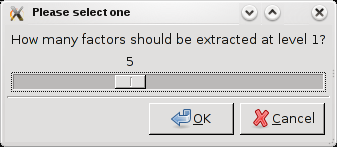
\includegraphics[width=2in]{screenshots2/simultaneous/fivefactors}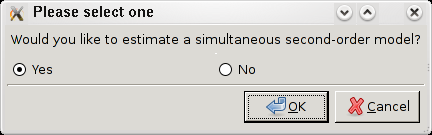
\includegraphics[width=2.5in]{screenshots2/simultaneous/yesno}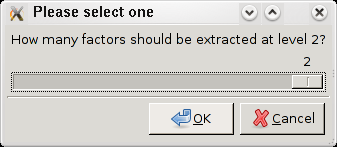
\includegraphics[width=2in]{screenshots2/simultaneous/twofactors}

Some people may be unfamiliar with the idea of a two-level model;
it is briefly defined in the Notation section and also in the help
page for \Rcode{make\_restrictions}. If $r\geq3$, the user will
be asked whether to estimate a simultaneous second-order model, which
decomposes the correlation matrix among first-order primary factors
$\left(\boldsymbol{\Phi}\right)$ as a function of fewer second-order
factors. For example, some people define ``general intelligence''
to be the second-order factor that drives various first-order (primary)
mental abilities. 

If a second-order model is estimated, and if $r\geq5$, the user will
be asked how many second-order factors $\left(\ddot{r}\right)$ to
extract. For the sake of completeness, I will assume that the user
answered ``Yes'' to the question of whether a simultaneous second-order
model should be estimated. Then, the dialog asks the user to specify
the number of second-order factors to extract. If $r=3$ or $r=4$,
then $\ddot{r}$ can only be one. If $r=5$, then $\ddot{r}$ can
be one or two. If $r\geq7$, then $\ddot{r}$ can be three in a SEFA
model. Rarely would one need to estimate a model with larger numbers
for $r$ and $\ddot{r}$. I will assume that the user has chosen $\ddot{r}=2$.


\subsection{Main menu}

The following menu is is critical in the sense that the user will
only be subsequently asked about options that are checked. This menu
would have fewer options if there were no simultaneous second-order
model, or if there were only one second-order factor, or if the model
were a CFA. It is quite possible to check multiple options. I will
discuss each of these options eventually; however, the order in which
subsequent options are specified is not necessarily the same order
that is presented in this menu.

\noindent \begin{center}
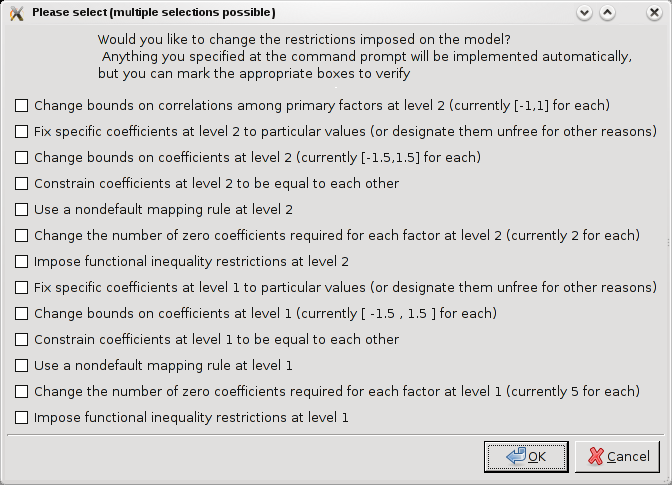
\includegraphics[width=6.5in]{screenshots2/menunator}
\par\end{center}


\subsubsection{Fix specific coefficients to particular values (second and eigth
checkboxes)}

The figures below illustrate dialogs that ask about pegging specific
coefficients to particular values \emph{a priori} and hence not estimating
them. The dialogs for both level two $\left(r\times\ddot{r}\right)$
and level one $\left(n\times r\right)$ are shown simultaneously here
but are not actually simultaneously specified when using FA$i$R.
Although it is not visably apparent unless the editor window is maximized,
the dimensions of matrix to be edited are the same as the dimensions
of the matrix to eventually be estimated, and there is an exact correspondence
between the cells of the editor window and the cells of $\boldsymbol{\beta}$
(or $\ddot{\boldsymbol{\beta}}$ as the case may be). This correspondence
holds in almost all of the editor windows to follow, but this matrix-based
interface may not be as intuitive to users who are accustomed to specifying
SEMs with path diagrams. Although this example is a SEFA, these dialogs
are more characteristic of a CFA model, which requires enough \emph{a
priori} zero coefficients to satisfy the theorems discussed in section
\ref{sub:Howe}. If this were a CFA model, these editing windows would
pop up regardless of whether the user requested so.

\noindent \begin{center}
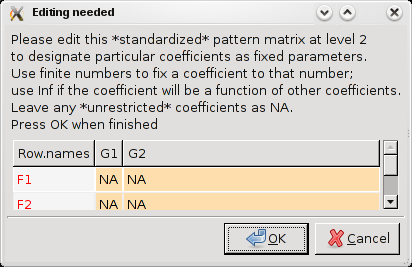
\includegraphics[width=3in]{screenshots2/peg_coefficients/peg_coefficients2}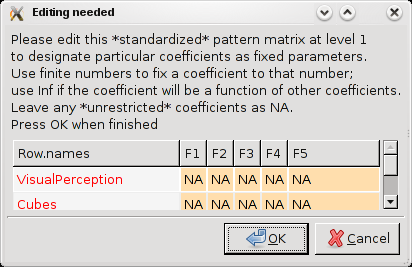
\includegraphics[width=3in]{screenshots2/peg_coefficients/peg_coefficients1}
\par\end{center}

There are several important things to note. First, any unrestricted
coefficients should be left as \Rcode{NA}. In many SEM programs,
a coefficient is restricted to be zero unless the user specifies otherwise.
This is \emph{not} the case in FA$i$R; if and only if you specify
that a coefficient is zero will it be zero \emph{a priori}. In a SEFA
model, it is possible to leave all cells as \Rcode{NA}, but doing
so would generate an error message under a CFA model.

Second, in many SEM programs it is possible or even customary to specify
that some coefficient is $1.0$ to normalize the scale of a factor.
In FA$i$R, the user generally should \emph{not} restrict one coefficient
per factor to have a coefficient of $1.0$ because the factors are
already normalized to have unit variances along the diagonal of $\boldsymbol{\Phi}$.
Hence, to also constrain a coefficient to be $1.0$ would be a substantive
restriction rather than merely a normalization.

Third, if one were to restrict a coefficient to be $1.0$, then one
would almost always restrict the other coefficients in that row to
be $0.0$, in which case the corresponding outcome variable will be
treated as {}``exogenous'' and its standard deviation will be estimated
from the data rather than by the model. Hence, this mechanism (which
is apparently all too familiar to long-time users of LISREL) can be
used for factor analysis where some factors are identical to observed
manifest variables. However, this specification is not generally recommended
in FA$i$R. It is better to exploit a feature of FA$i$R (discussed
below) to designate some outcome variable as the {}``best'' (yet
imperfect) indicator of a factor.

Fourth, if one wanted to impose the restriction that some coefficient
is an exact function of other coefficients (but not the simpler restriction
that two or more coefficients are equal), then it is necessary to
designate the {}``fixed'' coefficient in this dialog and pass a
function that enforces these restrictions to the \Rcode{nl\_1} or
\Rcode{nl\_2} arguments of \Rcode{make\_restrictions}. For example,
to impose the restriction that the first coefficient on the {}``Visual
Perception'' test is the ratio of the second and third coefficients,
one could proceed like this \Rcode{\\foo <- function(x) \{\\
  x[1,1] <- x[1,2] / x[1,3]\\
  return(x)\\
\}\\res <- make\_restrictions(manifest = man, model = "SEFA", nl\_1 = foo)\\}But it is also necessary to designate $\beta_{11}$ as {}``fixed'',
even though we do not know what number it is fixed to until $\beta_{12}$
and $\beta_{13}$ are specified. In such situations, {}``fix'' coefficients
that are exact functions of other coefficients to \Rcode{Inf} (note
the capitalization of \Rcode{Inf}).

Fifth, if merely imposing the restriction that two or more coefficients
are equal to each other, do not pass such a function to \Rcode{nl\_1}
or \Rcode{nl\_2} and do not bother designating affected coefficients
as {}``fixed'' in this dialog. Instead, use the dedicated mechanism
for imposing equality restrictions, which is discussed in the next
subsection. 

All that said, the most common use of this dialog (particularly for
a CFA) is to restrict specific coefficients to be $0.0$. Simply type
$0.0$ in the appropriate cell(s), \textit{press Enter to make sure
the change {}``registers'' in the editor}, and press OK to exit
this dialog. If restricting a specific coefficient to some number
other than $0.0$, keep in mind that the embedded correlation parameterization
in FA$i$R means that coefficients are calibrated for \emph{standardized}
variables.


\subsubsection{Constrain coefficients to be equal to each other (fourth checkbox)}

This figure illustrates the dialog to constrain one or more coefficients
(at level one) to be equal to each other; the dialog for level two
is similar. Again, it is not visibly apparent unless the editor window
is maximized but the dimensions of the matrix to be edited are $n\times r$
just like $\boldsymbol{\beta}$. 

\noindent \begin{center}
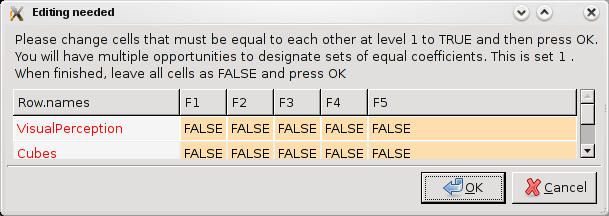
\includegraphics{screenshots2/equalities/equalities}
\par\end{center}

The matrix is initially filled with \Rcode{FALSE}, which is a keyword
in R. To impose an equality restriction among two or more coefficients,
change at least two of the cells to \Rcode{TRUE}, which is also a
keyword in R. \textit{The capitalization is essential}. For example,
to impose the restriction that $\beta_{11}=\beta_{21}$, I would change
the first two cells in the first column to \Rcode{TRUE}. It is possible
to constrain three or more coefficients to all be equal to each other
by changing three or more cells to \Rcode{TRUE}. When all cells that
are restricted to be equal to each other are designated with \Rcode{TRUE}
in the appropriate cell, click OK.

At that point, all the cells will be reset to \Rcode{FALSE}, which
allows you to impose \emph{another} set of equality restrictions (among
a disjoint set of coefficients, e.g. $\beta_{14}=\beta_{15}$). This
process can be repeated as many times as is necessary to represent
all the equality coefficients you want to impose on disjoint sets
of coefficients. If OK is clicked when all cells remain \Rcode{FALSE},
then whatever dialogue box is next appears.

Finally, again recall that the embedded correlation parameterization
in FA$i$R implies that coefficients should be calibrated for standardized
variables. Hence, constraining two or more cells of $\boldsymbol{\beta}$
to be equal does not imply that the corresponding cells of $\boldsymbol{\Omega}\boldsymbol{\beta}$
will be equal.


\subsubsection{Change bounds on coefficients (third checkbox)}

These figures ask about bounds on coefficients at level one, i.e.
on $\boldsymbol{\beta}$. The dialogue for level two would be similar.

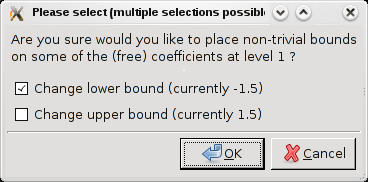
\includegraphics{screenshots2/bounds_coefficients/sure}\\
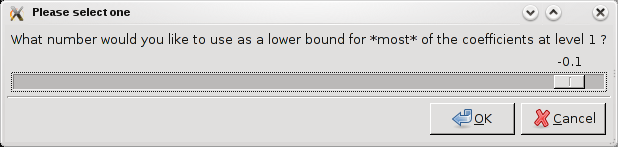
\includegraphics{screenshots2/bounds_coefficients/slider}\\
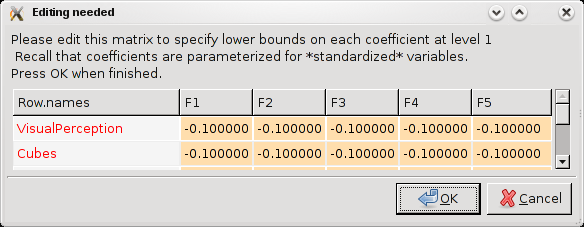
\includegraphics{screenshots2/bounds_coefficients/editor}

Specifying bounds on coefficients is a three-stage process. First,
the user is asked whether to change the lower and / or upper bounds
from their default values, here $\pm1.5$. I only illustrate changing
the lower bounds, but the process is similar if one wanted to additionally
or alternatively change the upper bounds.

Second, the user is asked for a {}``fill value'' to use for \emph{most}
of the (lower in this case) bounds on coefficients. After pressing
OK, this value is filled into an editable matrix that is of the same
dimension as $\boldsymbol{\beta}$, although that is not obvious when
the editor window is not maximized. Third, the user can edit any cell
of this $n\times r$ matrix to modify the bound for any coefficient.
Here I leave all lower bounds at my {}``fill value'' of $-0.1$.
Thus, this model requires a {}``almost-positive'' manifold, which
is a \emph{substantive} constraint that can be wrong and can be tested.

Finally, again recall that the embedded correlation parameterization
in FA$i$R implies that coefficients (and hence their bounds) should
be calibrated for standardized variables. In particular, rarely would
it be necessary to make the bounds \emph{wider} than $\pm1.5$ because
more extreme standardized coefficients are incredibly rare (provided
that $\boldsymbol{\Phi}$ is well-conditioned). Moreover, if there
were only one factor, it is impossible to make the bounds on its coefficients
wider than $\pm1.0$. If one were to impose the inequality restriction
that there are no negative suppresor variables (see below), then it
is somewhat advantageous to also narrow the upper bound on the coefficients
to $1.0$.


\subsubsection{Important Note}

The running example is a two-level model. In two-level models, one
cannot currently impose bounds on the off-diagonals of $\boldsymbol{\Phi}$
using the pop-up menus. However, if this were a one-level model, the
next dialog box would ask about bounds on the off-diagonals of $\boldsymbol{\Phi}$
if such an option were selected from the main menu. That dialog would
be similar to the one illustrated in subsubsection \ref{sub:bounds_cormat}.


\subsubsection{Nondefault mapping rule and changing the requisite number of zeros
(11th and 12th checkboxes)\label{sub:mapping_rule}}

In the SEFA model presumed here, the question shown in the figure
below is very important and pertains to the mapping rule used to squash
certain cells of $\boldsymbol{\beta}$ to zero during the optimization.
The dialog for level two is similar but generally has fewer options.
If a CFA model were being estimated, this question would not appear
because the theorems in section \ref{sub:Howe} must be satisfied
by \emph{a priori} restrictions. Specifying a non-default mapping
rule is more common for a rather {}``exploratory'' SEFA; for a more
{}``confirmatory'' SEFA, one would typically accept the default
mapping rule and suppliment it with other restrictions.

\noindent \begin{center}
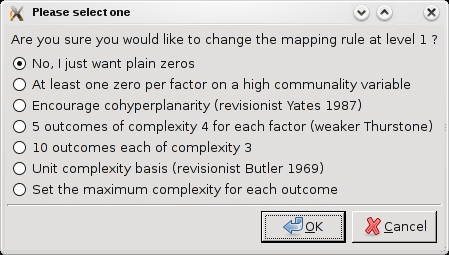
\includegraphics{screenshots2/mapping_rule/sure}
\par\end{center}

Let $b_{p}$ be the number of zeros required for the $p$th column
of $\boldsymbol{\beta}$. Let $\underline{\boldsymbol{\beta}}$ be
a matrix with the same dimensions as $\boldsymbol{\beta}$. Suppose
the free cells of $\underline{\boldsymbol{\beta}}$ have been filled
in by a proposal for the restricted optimum of the discrepancy function,
but it has fewer than $b_{p}$ zeros in the $p$th column (and possibly
no zeros at all). The {}``mapping rule'' maps from $\underline{\boldsymbol{\beta}}$
to $\boldsymbol{\beta}$ by changing some {}``small'' cells of $\underline{\boldsymbol{\beta}}$
to zero and then the discrepancy function (and each constraint function)
is evaluated at $\boldsymbol{\beta}$, not $\underline{\boldsymbol{\beta}}$
. By {}``small'', I always mean in absolute value; however the rules
are usually defined on the reference structure matrix $\left(\underline{\boldsymbol{\Upsilon}}=\underline{\boldsymbol{\beta}}\mathbf{D}\right)$
or the factor contribution matrix $\left(\boldsymbol{\Game}=\underline{\boldsymbol{\beta}}\times\left(\underline{\boldsymbol{\beta}}\boldsymbol{\Phi}\right)\right)$
, rather than $\underline{\boldsymbol{\beta}}$ itself.
\begin{itemize}
\item ``No, I just want plain zeros''. This default mapping rule simply
squashes the $b_{p}$ smallest elements in $\underline{\boldsymbol{\beta}_{p}}$
to zero.
\item {}``At least one zero per factor on a high communality variable.''
This mapping rule is similar but is slightly more complicated. Let
$\overline{\Game_{j}}=\frac{1}{r}\sum_{p=1}^{r}\underline{\Game_{jp}}=\frac{h^{2}}{r}$
be the arithmetic mean of the factor contributions for the $j$th
outcome variable and let $\widetilde{\Game_{j}}=\left(\prod_{j=1}^{r}\underline{\Game_{jp}}\right)^{\frac{1}{r}}$
be the geometric mean of the factor contributions for the $j$th outcome,
which is defined only for outcomes with nonnegative factor contributions.
Hence, $\frac{\overline{\Game_{j}}}{\widetilde{\Game_{j}}}$ will
tend to be more positive when the communality of the $j$th outcome
is large but at least one factor contributes little to the communality.
Define the set of {}``potential zeros'' on factor $p$ as those
rows of $\underline{\boldsymbol{\Upsilon}}$ where $\underline{\Upsilon_{jp}}<\underline{\Upsilon_{jq}}\,\forall q\neq p$.
For each $p$, this mapping rule squashes $\underline{\beta_{jp}}$
to zero for the outcome among the set of {}``potential zeros'' with
the largest (well-defined) $\frac{\overline{\Game_{j}}}{\widetilde{\Game_{j}}}$.
The default mapping rule is then applied to squash $b_{p}-1$ more
cells to zero for the $p$th factor.
\item ``Encourage cohyperplanrity (revisionist Yates 1987)''. This very
promising mapping rule squashes $r-1$ cells in the $p$th column
of $\underline{\boldsymbol{\beta}}$ using the following piecewise
function $\forall q\neq p$:\begin{eqnarray*}
\beta_{jp} & = & \begin{cases}
0 & \textrm{if}\,\underline{\Game_{jq}}-\underline{\Game_{jp}}=\max\left\{ \underline{\boldsymbol{\Game}_{q}}-\underline{\boldsymbol{\Game}_{p}}\right\} \\
\underline{\beta_{jp}} & \textrm{otherwise,}\end{cases}\end{eqnarray*}
which tends to place the zeros for the $p$th column of $\boldsymbol{\beta}$
in the rows where the factor contribution of the $q$th factor is
large. The default mapping rule is then applied to squash $b_{p}-\left(r-1\right)$
more cells to zero for the $p$th factor. Although Yates (1987) did
not anticipate SEFA, it repeatedly recommends procedures that tend
to encourage outcomes within hyperplanes in the common factor space
to be widely dispersed throughout their hyperplane(s). This mapping
rule attempts to do so.
\item ``$r$ outcomes of complexity $r-1$ for each factor (weaker Thurstone)''.
This mapping rule is similar to the default mapping rule in that $r$
small elements in the $p$th column of $\boldsymbol{\beta}$ are squashed
to zero, except that there is an additional stipulation that no outcome
is of complexity less than $r-1$ where the complexity of the $j$th
outcome is its number of non-zero coefficients. However, any ``non-zero''
coefficient can be arbitrarily close to zero. Thus, each column of
$\boldsymbol{\beta}$ will have $r$ \emph{exact} zeros. If necessary,
the default mapping rule will then be applied to squash $b_{p}-r$
more cells to zero for the $p$th factor.
\item {}``$2r$ outcomes each of complexity $r-2$.'' This mapping starts
by finding the smallest cell in the first column of $\underline{\boldsymbol{\Upsilon}}$
and squashes it to zero. Say this cell is $\underline{\Upsilon_{j1}}$.
Then, the smallest nonzero cell in the $j$th row of $\underline{\boldsymbol{\Upsilon}}$
is also squashed to zero so that the $j$th outcome is of complexity
$r-2$. This procedure is repeated for all columns to yield $2r$
outcomes each of complexity $r-2$, such that each factor has $r-1$
zeros. Finally, the default mapping rule is applied to squash $b_{p}-\left(r-1\right)$
more cells to zero for the $p$th factor.
\item ``Unit complexity basis (revisionist Butler 1969)''. Butler (1969)
defines {}``the $r$ most distinguished outcomes'' and proposes
to run the $r$ primary axes through them in EFA to create a unit
complexity basis for $\boldsymbol{\beta}$. The following SEFA mapping
rule is similar and is defined by a piecewise function $\forall q\neq p$:
\begin{eqnarray*}
\beta_{jp} & = & \begin{cases}
0 & \textrm{if\ensuremath{\,}}\textrm{abs}\left(\underline{\beta_{jq}}\right)=\max\left(\textrm{abs}\left(\underline{\boldsymbol{\beta}_{q}}\right)\right)\\
\underline{\beta_{jp}} & \textrm{otherwise}\end{cases}\end{eqnarray*}
The default mapping rule is then applied to squash $b_{p}-\left(r-1\right)$
more cells to zero for the $p$th factor.
\item {}``Set the maximum complexity for each outcome.'' This mapping
rule is similar to the default mapping rule, except that it is applied
to the \emph{rows} of $\boldsymbol{\Upsilon}$ rather than its columns.
In general, $\forall j$, the user can choose $b_{j}\in\left\{ 0,\dots,r-1\right\} $
for the minimum number of zero coefficients in $\boldsymbol{\beta}_{j}$,
and the complexity of the $j$th outcome is $r-b_{j}$. It is possible
to choose the same complexity for all rows of $\boldsymbol{\beta}$.
If the complexity of $\boldsymbol{\beta}_{j}$ is $r-1\,\forall j$,
this restriction characterizes the main tenet of Thurstone's (1935)
definition of simple structure. If the complexity of $\boldsymbol{\beta}_{j}$
is $1\,\forall j$, this restriction implies a perfect cluster configuration.
Alternatively, $b_{j}$ can be specified on a row-by-row basis, as
is shown in the dialog below, which will pop up if this maping rule
is selected. Finally, the default mapping rule is applied to ensure
that there are at least $b_{p}$ zeros for the $p$th factor.
\end{itemize}
\noindent \begin{center}
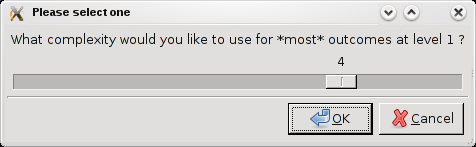
\includegraphics[width=3.25in]{screenshots2/mapping_rule/slider}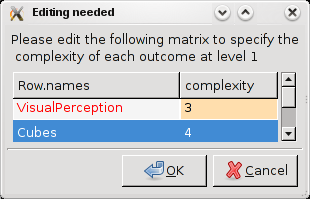
\includegraphics[width=3.25in]{screenshots2/mapping_rule/complexity}
\par\end{center}

Finally, in the case of SEFA, it is necessary to specify $b_{p}\,\forall p$.
By default, $b_{p}=r\,\forall p$, which is the minimum that is necessary
for identification of the nonzero parameters. However, it is possible
to select $b_{p}>r$ and may be possible to select $b_{p}=r-1$ in
some cases if identification of the relevant parameters can be accomplished
in some other fashion. The following dialogs illustrate this mechanism,
which is initialized when the box for {}``Change the number of zero
coefficients required for each factor'' is checked in the main menu:

\noindent \begin{center}
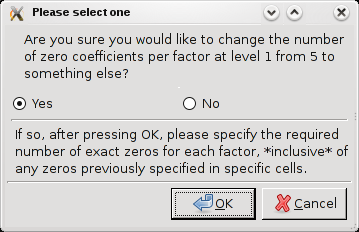
\includegraphics[width=3.5in]{screenshots2/zeros/sure}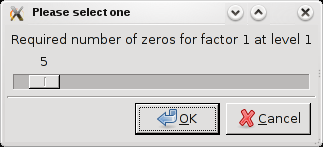
\includegraphics[width=3in]{screenshots2/zeros/slider}
\par\end{center}


\subsubsection{Change bounds on correlations among primary factors (first checkbox)\label{sub:bounds_cormat}}

This figure below illustrates a dialog that asks about bounds on the
off-diagonals of $\ddot{\boldsymbol{\Phi}}$. If $\ddot{r}\leq1$,
this question would not be asked, although if $\ddot{r}=0$, a similar
dialogue would ask about bounds on the off-diagonals of $\boldsymbol{\Phi}$.
If there were more factors, the editor window would have more rows,
totalling $0.5\ddot{r}\left(\ddot{r}-1\right)$.

The user is given an editor with columns for the lower and upper bounds
on these correlations. The bounds cannot exceed $\pm1$ because they
pertain to correlations. Here, I edited the admissable interval to
$\left[-0.9,0.9\right]$, which is a largely irrelevant restriction.

\noindent \begin{center}
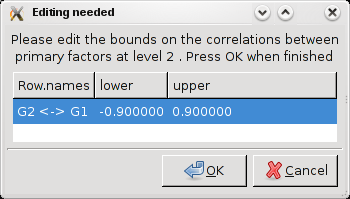
\includegraphics[height=2.5in]{screenshots2/bounds_cormat/bounds_cormat}
\par\end{center}


\subsubsection{Impose functional inequality restrictions\label{sub:funky}}

It is always important to keep in mind that FA$i$R does something
tantamount to restricted optimization and that the possibilities for
restrictions are endless. Hence, perhaps the most important feature
of FA$i$R is the ability to impose inequality restrictions on functions
of multiple parameters. It is even possible to define your own restriction
functions and pass them to the criteria argument of \Rcode{make\_restrictions}.
In this subsection, I will only discuss the functional inequality
restrictions that are pre-programmed in FA$i$R. 

Please refer to section \ref{sec:definitions} for definitions of
the factor contribution matrix, the generalized variance, and the
effective variance. Also, let $\mathbb{I}\left\{ \cdot\right\} $
be the {}``indicator function'', which equals $1$ if the condition
inside the braces is true and equals $0$ if the condition is false.
In FA$i$R, an inequality restriction function is a piecewise function
that equals $-1$ if the restriction is satisfied and equals some
number greater than $-1$ if the the restriction is not satisfied.
You do not need to worry too much about the return values for the
case where the restriction is not satisfied.

When the box for {}``Impose functional inequality restrictions''
(at level one) is checked, the following menu appears:

\noindent \begin{center}
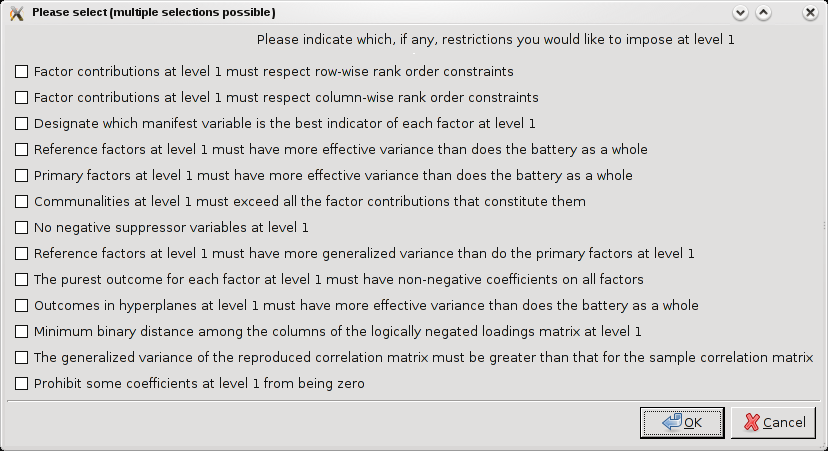
\includegraphics[width=6.5in]{screenshots2/constraints/menu}
\par\end{center}

The menu would be similar at level two but will perhaps have fewer
options. These restrictions are defined as follows:
\begin{itemize}
\item {}``Factor contributions must respect row-wise order constraints.''
Let $\mathbf{G}$ be a $n\times r$ matrix that is specified by the
user to indicate the required ranks of the factor contributions within
each row with larger factor contributions receiving smaller ranks.
For example, $\mathbf{G}_{j}$ could be $\begin{bmatrix}4 & 1 & 5 & 3 & 2\end{bmatrix}$
to require that the second factor contribution in the $j$th row be
biggest, the third factor contribution be smallest, etc. However,
it is not necessary for the ranks to be unique. For example, $\mathbf{G}_{j}$
could be $\begin{bmatrix}5 & 1 & 5 & 5 & 5\end{bmatrix}$ to require
that the second factor contribution in the $j$th row be biggest,
while allowing the other ranks to be unrestricted. Such a specification
would often be used in CFA or in a more {}``confirmatory'' SEFA
where the user has strong theoretical reason to believe that the $j$th
outcome largely {}``measures'' the $p$th factor and thus specifies
that $G_{jp}=1$ and that $G_{jq}=r\,\forall q\neq p$. But keep in
mind that, for example, $\mathbf{G}_{j}=\begin{bmatrix}2 & 2 & 5 & 5 & 5\end{bmatrix}$
is also valid and requires that the first two factor contributions
in the $j$th row be the top two without taking a position on whether
the first is larger than the second. Conversely, $\mathbf{G}_{j}=\begin{bmatrix}2 & 2 & 3 & 3 & 5\end{bmatrix}$,
for example, is invalid because it is impossible for the first four
factor contributions to all be ranked in the top three.\\
$\mathbf{G}$ can be specified interactively in response to the
following dialog:%
\footnote{This restriction can also be enforced from the command line with \Rcode{make\_restrictions(*, critieria = list("ranks\_rows\_1st"), methodArgs = list(row\_ranks\_1st = G))}where
$\mathbf{G}$ matrix is manually defined in the global environment.%
}\\
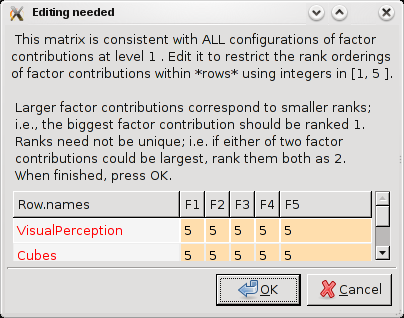
\includegraphics{screenshots2/constraints/rowranks}\\
 Let $\underrightarrow{\boldsymbol{\Game}}$ be a factor contribution
matrix that has been converted to ranks within rows. The function
that imposes this constraint is formally defined as\begin{eqnarray*}
\frac{-1}{nr}\sum_{j=1}^{n}\sum_{p=1}^{r}\mathbb{I}\left\{ \underrightarrow{\Game_{jp}}\leq G_{jp}\right\}  & \in & \left[-1,0\right]\end{eqnarray*}
and thus equals $-1$ if and only if $\underrightarrow{\boldsymbol{\Game}}$
is consistent with $\mathbf{G}$ in every cell.
\item {}``Factor contributions must respect column-wise order constraints.''
Essentially, this constraint involves the same concept as the previous
constraint, except that $\underrightarrow{\boldsymbol{\Game}}$ and
$\mathbf{G}$ are defined on the basis of column-wise ranks. I use
the same notation as before but the matrices have different contents.
For example, $\mathbf{G}_{p}^{\prime}=\begin{bmatrix}3 & 3 & 3 & n & \dots & n\end{bmatrix}$
would require that the first three outcomes have the three largest
factor contributions on the $p$th factor. The remaining $n-3$ outcomes
can be ranked in any fashion on the $p$th factor, provided that none
is in the top three. Again, this mechanism would most often be used
in CFA or in a more {}``confirmatory'' SEFA. It is tempting to specify
that $G_{jp}=1$ in order to make the $p$th factor closely related
the to $j$th outcome, but there is a better mechanism for doing so,
which is discussed next.\\
$\mathbf{G}$ can be specified interactively in response to the
following dialog:%
\footnote{This restriction can also be enforced from the command line with \Rcode{make\_restrictions(*, critieria = list("ranks\_cols\_1st"), methodArgs = list(col\_ranks\_1st = G))}where
$\mathbf{G}$ matrix is manually defined in the global environment.%
}\\
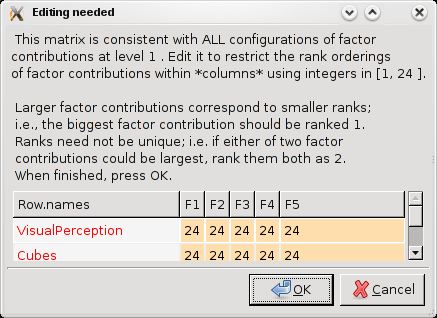
\includegraphics{screenshots2/constraints/colranks}\\
Let $\underrightarrow{\boldsymbol{\Game}}$ be a factor contribution
matrix that has been converted to ranks within columns. The function
that imposes this constraint is formally defined as\begin{eqnarray*}
\frac{-1}{nr}\sum_{j=1}^{n}\sum_{p=1}^{r}\mathbb{I}\left\{ \underrightarrow{\Game_{jp}}\leq G_{jp}\right\}  & \in & \left[-1,0\right]\end{eqnarray*}
and thus equals $-1$ if and only if $\underrightarrow{\boldsymbol{\Game}}$
is consistent with $\mathbf{G}$ in every cell.
\item {}``Designate which outcome variable is the best indicator of each
factor.'' This criterion just is a special case of the previous one
but is operationalized differently for better computational performance.
In essence, one is merely requiring that $G_{jp}=1$ and $G_{kp}=n\,\forall k\neq j$
for any designated $p$. Hence, it is not necessary to impose such
a restriction for every factor. This restriction would be used when
the user believes that the $j$th outcome is the $p$th factor but
measured with error. It may be fruitful to combine this restriction
with the restriction that $\beta_{jq}=0\,\forall q\neq p$ but doing
so is not required. Thus, this restriction is weaker and presumably
more realistic than the restriction that the $j$th variable is {}``exogenous''
and measured without error, i.e.~$\beta_{jp}=\mathbb{I}\left\{ q=p\right\} $.\\
 These indicators can be specified interactively in response to
the following dialog:%
\footnote{This restriction can also be enforced from the command line with \Rcode{make\_restrictions(*, criteria = list("indicators\_1st"), methodArgs = list(indicators\_1st = z))},
where \Rcode{z} is an integer vector with $r$ elements, each of
which contains the row number of the best indicator of the $p$th
factor, which can be \Rcode{NA\_integer\_} to avoid constraining
the $p$th factor.%
}\\
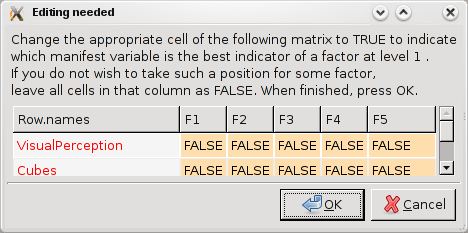
\includegraphics{screenshots2/constraints/indicators}\\
The function that imposes this constraint is formally defined as
as the average column-wise rank of the designated indicators (among
factors with designated indicators) less two. This function ranges
from $-1$ to $n-2$ and equals $-1$ if and only if the indicators
have the largest factor contribution in their respective columns.
\item {}``Reference factors at level 1 must have more effective variance
than does the battery as a whole''. The function that imposes this
constraint is formally defined as%
\footnote{This constraint can be enforced by from the command line with \Rcode{make\_restrictions(*, criteria = list("ev\_RF\_1st"))}. %
}\begin{eqnarray*}
\begin{cases}
-1 & \textrm{if\ensuremath{\,}}\left|\boldsymbol{\Psi}\right|^{\frac{1}{r}}\geq\left|\mathbf{R}\right|^{\frac{1}{n}}\\
\left|\mathbf{R}\right|^{\frac{1}{n}}-\left|\boldsymbol{\Psi}\right|^{\frac{1}{r}} & \textrm{otherwise}\end{cases} & \in & \left[-1,1\right],\end{eqnarray*}
This criterion loosely implies that the reference factors at level
1 be {}``less correlated'' than is the configuration of outcomes
in common factor space and encourages the primary axes to cut through
the edges of the test configuration. This restriction is extremely
weak and could be imposed in a more {}``exploratory'' SEFA.
\item {}``Primary factors at level 1 must have more effective variance
than does the battery as a whole''. The function that imposes this
constraint is formally defined as%
\footnote{This constraint can be enforced by from the command line with \Rcode{make\_restrictions(*, criteria = list("ev\_PF\_1st"))}. %
}\begin{eqnarray*}
\begin{cases}
-1 & \textrm{if\ensuremath{\,}}\left|\boldsymbol{\Phi}\right|^{\frac{1}{r}}\geq\left|\mathbf{R}\right|^{\frac{1}{n}}\\
\left|\mathbf{R}\right|^{\frac{1}{n}}-\left|\boldsymbol{\Phi}\right|^{\frac{1}{r}} & \textrm{otherwise}\end{cases} & \in & \left[-1,1\right],\end{eqnarray*}
and is similar to the previous criterion above except is more intuitive
because the effective variance of the primary factors is at issue.
In general, it seems that imposing this restriction on the primary
factors is \emph{stronger} than imposing it on the reference factors
and tends to push the first-order axes farther out into the edges
of the test configuration. It seems clear that Yates (1987) would
have supported this restriction but does not specifically mention
it.
\item {}``Communalities must exceed all the factor contributions that constitute
them.'' The function that imposes this constraint is formally defined
as%
\footnote{This constraint can be enforced by from the command line with \Rcode{make\_restrictions(*, criteria = list("h2\_over\_FC\_1st"))}. %
} \begin{eqnarray*}
\frac{-1}{nr}\sum_{j=1}^{n}\sum_{p=1}^{r}\mathbb{I}\left\{ h_{j}^{2}\geq\Game_{jp}\right\}  & \in & \left[-1,0\right],\end{eqnarray*}
which permits some negative suppressor variables but prohibits extreme
situations such as that where one factor contribution is large and
positive and another in that row is almost equally large in magnitude
but negative. Overall, this restriction seems quite weak.
\item {}``Best indicator of each factor must have non-negative factor contributions.''
Let $\underleftrightarrow{\boldsymbol{\Game}}$ be the $r\times r$
submatrix of $\boldsymbol{\Game}$ whose rows contain the best indicators
of each factor as defined by the column-maximums of $\boldsymbol{\Game}$
with the additional proviso that the rows are unique. The function
that imposes this constraint is formally defined as%
\footnote{This constraint can be enforced from the command line with \Rcode{make\_restrictions(*, criteria = list("distinguishability\_1st")}. %
}\begin{eqnarray*}
\frac{-1}{r^{2}}\sum_{q=1}^{r}\sum_{p=1}^{r}\mathbb{I}\left\{ \underleftrightarrow{\Game_{qp}}\geq0\right\}  & \in & \left[-1,0\right],\end{eqnarray*}
and is stronger than the previous criterion and weaker than the next
criterion. Although it prohibits negative suppressor variables among
the best indicators, it permits any degree of suppression among the
other outcome variables.
\item {}``No negative suppressor variables.'' Let $\Game^{\ast}\leq0$
be the minimum factor contribution that the user is willing to accept,
and thus wants all factor contributions to exceed this threshold to
prohibit {}``negative'' suppressor variables but perhaps make some
allowance for factor contributions to be slightly negative by chance.
This constraint can be specified interactively via the following diaglog
with $\Game^{\ast}=-0.01$:%
\footnote{This constraint can be enforced at the command line with \Rcode{make\_restrictions(*, criteria = list("no\_neg\_suppressors\_1st"), methodArgs = list(FC\_threshold\_1st = -.01))} %
}\\
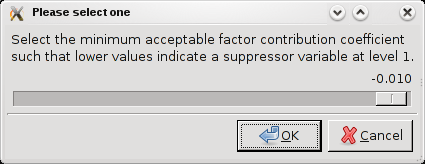
\includegraphics{screenshots2/constraints/nns}\\
The function that imposes this constraint is formally defined as\begin{eqnarray*}
\frac{-1}{nr}\sum_{j=1}^{n}\sum_{p=1}^{r}\mathbb{I}\left\{ \Game_{jp}\geq\Game^{\ast}\right\}  & \in & \left[-1,0\right],\end{eqnarray*}
and is a fairly strong --- yet in many cases, reasonable --- restriction.
Yates (1987, p.~119) essentially recommends it, albeit with some
incorrect statements about the relationship between this restriction
and the rest of the surrounding chapter.
\item ``Reference factors must have more generalized variance than do primary
factors''. The function that imposes this constraint could be formally
defined as%
\footnote{This constraint can be enforced by from the command line with \Rcode{make\_restrictions(*, criteria = list("gv\_1st"))}. %
} \begin{eqnarray*}
\begin{cases}
-1 & \textrm{if\ensuremath{\,}}\left|\boldsymbol{\Phi}\right|\leq\left|\boldsymbol{\Psi}\right|\\
\left|\boldsymbol{\Phi}\right|-\left|\boldsymbol{\Psi}\right| & \textrm{otherwise}\end{cases} & \in & \left[-1,1\right]\end{eqnarray*}
but has a faster and substantively equivalent operationalization in
the code. When $r_{1}=2$, $\left|\boldsymbol{\Phi}\right|=\left|\boldsymbol{\Psi}\right|$
by necessity, so this criterion can bind in the case when $r\geq3$.
Also, this criterion necessarily holds when there is a single second-order
factor. Yates (1987, p.~27) asserts that this restriction is a necessary
condition of a useful factor analysis model, although counter-examples
can be generated. With randomly drawn correlations from a uniform
distribution on $\left[-1,1\right]$, $\boldsymbol{\Phi}$ is both
positive definite and satisfies this restriction about $25\%$ of
the time when $r=3$, $5\%$ of the time when $r=4$, $0.5\%$ of
the time when $r=5$, and even less frequently for $r>5$. 
\item ``Outcomes in hyperplanes have more effective variance than does the
battery as a whole''. The function that imposes this constraint is
formally defined as%
\footnote{This constraint can be enforced from the command line with \Rcode{make\_restrictions(*, criteria = list("cohyperplanarity\_1st"))}. %
} \begin{eqnarray*}
\frac{-1}{r}\sum_{p=1}^{r}\mathbb{I}\left\{ \left|\overset{p}{\boldsymbol{\beta}}\boldsymbol{\Phi}\overset{p}{\boldsymbol{\beta}^{\prime}}+\overset{p}{\boldsymbol{\Theta}^{2}}\right|^{\frac{1}{b_{p}}}\geq\left|\mathbf{R}\right|^{\frac{1}{n}}\right\}  & \in & \left[-1,0\right],\end{eqnarray*}
where $\overset{p}{\boldsymbol{\beta}}$ is the $b_{p}\times r$ submatrix
of $\boldsymbol{\beta}$ with exact zeros in the $p$th column and
$\overset{p}{\boldsymbol{\Theta}^{2}}$ is the $b_{p}\times b_{p}$
diagonal submatrix of $\boldsymbol{\Theta}^{2}$ with the unique variances
for these $b_{p}$ outcomes. Thus, this criterion loosely requires
that the outcomes in the $p$th hyperplane be ``less correlated''
than is the battery as a whole (in common factor space) for all $r$
hyperplanes and is thus fairly strong. This constraint goes well with
the revisionist Yates mapping rule discussed in section \ref{sub:mapping_rule}.
\item {}``Minimum binary distance among columns of the logically negated
loadings matrix.'' Let $\beta_{jp}^{\ast}=\begin{cases}
1 & \textrm{if}\,\beta_{jp}=0\\
0 & \textrm{if}\,\beta_{jp}\neq0\end{cases}$ be the {}``logically negated loadings matrix''. The binary distance
between two columns of the {}``logically negated loadings matrix''
is defined as (see \Rcode{?dist}) as {}``the \textit{proportion}
of bits in which only one is on amongst those in which at least one
is on''. In order to satisfy the theorem in Reiers\o{}l (1950),
the minimum binary distance betwen any two columns must be positive,
but it is possible to require a larger minimum binary distance. \\
Let $d^{\ast}$ be the requisite minimum binary distance, which
can be specified in response to the following dialog:\\
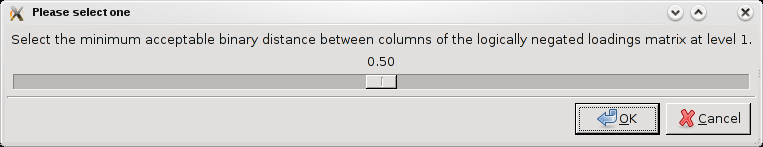
\includegraphics{screenshots2/constraints/distance}\\
Let $d_{qp}$ be the binary distance between the $q$th and $p$th
columns of $\boldsymbol{\beta}$. The function that imposes this constraint
is formally defined as%
\footnote{This constraint can also be enforced from the command line with \Rcode{make\_restrictions(*, critieria = list("dist\_cols\_1st"), methodArgs = list(cutpoint\_1st = 0.5))}%
}\begin{eqnarray*}
\frac{-2}{r\left(r-1\right)}\sum_{q=1}^{r}\sum_{p\neq q}^{r}\mathbb{I}\left\{ d_{qp}\geq d^{\ast}\right\}  & \in & \left[-1,0\right]\end{eqnarray*}
and would most often be used in a more {}``exploratory'' SEFA.
\item {}``Generalized variance of the reproduced correlation matrix must
be less than that of the sample correlation matrix.'' The function
that imposes this constraint is formally defined as%
\footnote{This constraint can be enforced from the command line with \Rcode{make\_restrictions(*, criteria = list("volume\_1st"))}. %
}\begin{eqnarray*}
\begin{cases}
-1 & \textrm{if\ensuremath{\,}}\left|\mathbf{R}\right|\geq\left|\textrm{cor}\left(\mathbf{Y}\right)\right|\\
\left|\textrm{cor}\left(\mathbf{Y}\right)\right|-\left|\mathbf{R}\right| & \textrm{otherwise}\end{cases} & \in & \left[-1,1\right],\end{eqnarray*}
where $\left|\textrm{cor}\left(\mathbf{Y}\right)\right|$ is the determinant
of the sample correlation matrix. This restriction is pretty weak.
\item {}``Prohibit some coefficients from being zero.'' This restriction
is relevant only for SEFA, where it is possible that the mapping rule
will map some coefficient to zero that theoretically should not be
zero. The most common case where this restriction is helpful is when
equality restrictions are impose on two coefficients, and one presumably
intends that they both be nonzero. The genetic algorithm would otherwise
tend to make both zero and thereby satisfy two restrictions the easy
way.\\
Let $\boldsymbol{\beta}^{\ast}$ be a matrix such that $\beta_{jp}^{\ast}=1$
if $\beta_{jp}$ must not be zero and equals zero otherwise, which
can be specified in response to the following dialog:\\
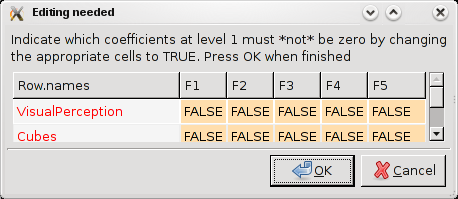
\includegraphics{screenshots2/constraints/blocks}\\
The function that imposes this constraint is formally defined as%
\footnote{This constraint can also be enforced at the command line with \Rcode{make\_restrictions(*, criteria = list("block\_1st"), methodArgs = list(blockers = beta\_star))}%
}\begin{eqnarray*}
\frac{-1}{\sum_{j=1}^{n}\sum_{p=1}^{r}\beta_{jp}^{\ast}}\sum_{j=1}^{n}\sum_{p=1}^{r}\mathbb{I}\left\{ \beta_{jp}^{\ast}=1\right\} \mathbb{I}\left\{ \beta_{jp}\neq0\right\}  & \in & \left[-1,0\right]\end{eqnarray*}
and equals $-1$ if and only if none of the prohibited coefficients
are zero.
\end{itemize}
Note that it is possible to select (or specify at the command line)
more than one of these criteria as constraints in the lexical optimization
process.\newpage{}


\section{Exploratory Factor Analysis via \texttt{Factnal()} and \texttt{Rotate()}}

To start this sequence, I typed the command\\
\Rcode{man <- make\_manifest(covmat = Harman74.cor)}\\
\Rcode{res <- make\_restrictions(manifest = man, factors = 5, model = "EFA")}\\
\Rcode{EFA <- Factanal(manifest = man, restrictions = res)}\\


\subsection{Factor Extraction}

I use $\boldsymbol{\Lambda}$ to indicate the preliminary pattern
matrix to estimate when the preliminary factors are orthogonal. The
above sequence of commands will estimate the EFA model under the assumptions
that $\boldsymbol{\Phi}=\mathbf{I}$ and that $\boldsymbol{\Lambda}^{\prime}\boldsymbol{\Theta}^{-2}\boldsymbol{\Lambda}$
is diagonal using the maximum likelihood discrepancy function. If
a different discrepancy function were specified, then the EFA model
would be estimated under the assumptions that $\boldsymbol{\Phi}=\mathbf{I}$
and that $\boldsymbol{\Lambda}=\begin{bmatrix}\boldsymbol{\Lambda}_{1}\\
\boldsymbol{\Lambda}_{2}\end{bmatrix}$ where $\boldsymbol{\Lambda}_{1}$ is a $r\times r$ matrix with zeros
above its diagonal. 


\subsection{Factor Transformation}

Note that regardless of how the EFA model was estimated, the preliminary
factors will have the noncanonical form where $\boldsymbol{\Lambda}=\begin{bmatrix}\boldsymbol{\Lambda}_{1}\\
\boldsymbol{\Lambda}_{2}\end{bmatrix}$ and $\boldsymbol{\Lambda}_{1}$ is a $r\times r$ matrix with zeros
above its diagonal. After verifying that a EFA model with $r$ factors
fits the data reasonably well, there were no near-Heywood cases, etc.,
the next task is to choose a transformation of the preliminary factors.

Let $\boldsymbol{\Phi}=\mathbf{T}^{\prime}\mathbf{T}$ where $\mathbf{T}$
is a $r\times r$ transformation matrix with unit-length columns (not
rows). The factor transformation step chooses $\mathbf{T}$ so so
that some (lexical) objective function is \textit{minimized}. I initiated
this sequence with\\ \Rcode{EFA\_rotated <- Rotate(EFA)}

\textbf{WARNING: The subsequent pop-up menus are presented here in
the logical order, which is different than the order in which they
will appear when calling \Rcode{Rotate()}.}


\subsubsection{Functional inequality restrictions}

Again let $\mathbb{I}\left\{ \cdot\right\} $ be the {}``indicator
function'', which equals $1$ if the condition within the braces
is true and equals $0$ if the condition is false. In FA$i$R, an
inequality restriction function is a piecewise function that equals
$-1$ if the restriction is satisfied and equals some number greater
than $-1$ if the the restriction is not satisfied. You do not need
to worry too much about the return values for the case where the restriction
is not satisfied.

One such inequality restriction is mandatory and is used to prevent
factor collapse. The function that imposes this constraint is formally
defined as\begin{eqnarray*}
\begin{cases}
-1 & \textrm{if\ensuremath{\,}}\left|\boldsymbol{\Phi}\right|^{\frac{1}{r}}\geq v^{\ast}\\
v^{\ast}-\left|\boldsymbol{\Phi}\right|^{\frac{1}{r}} & \textrm{otherwise}\end{cases} & \in & \left[-1,1\right],\end{eqnarray*}
where $v^{\ast}>0$ is the minimum acceptable effective variance for
the primary factors. Please refer to section \ref{sec:definitions}
for the definition of effective variance. One can specify $v^{\ast}$
by responding to the following dialog:%
\footnote{The corresponding pop-up menu can be avoided from the command line
with \Rcode{Rotate(EFA, criteria = list("no\_factor\_collapse"), methodArgs = list(nfc\_threshold = .3))}%
}

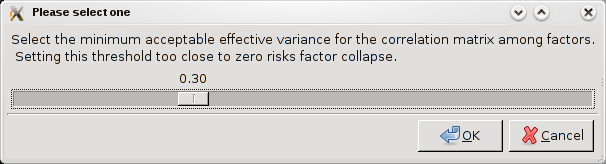
\includegraphics{screenshots2/EFA/nfc}

A value of $v^{\ast}=0.3$ is quite weak and in the $r=2$ case would
permit the off-diagonal of $\boldsymbol{\Phi}$ to be up to $\pm0.954$,
which only precludes \textit{literal} factor collapse. One deliberately
nice property of defining the restriction with respect to the effective
variance is that the same $v^{\ast}$ is more-or-less reasonable regardless
of $r$.

The following menu is similar to that in section \ref{sub:funky},
which offered choices for functional inequality restrictions on SEFA
and CFA models. Except for the first two choices, the definitions
of the criteria and subsequent pop-up menus are the same; only the
two that differ will be discussed in this subsection.

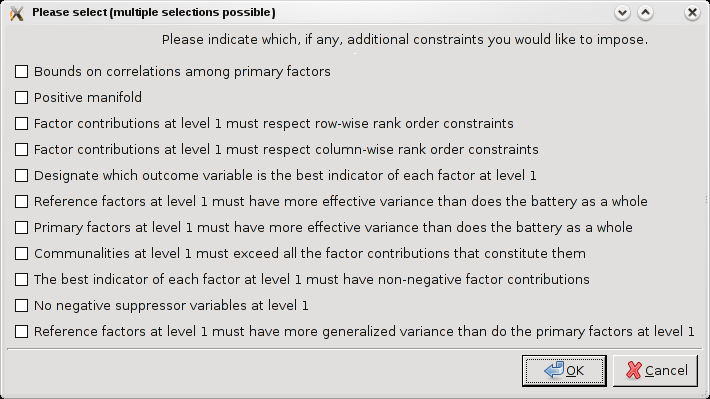
\includegraphics[width=6.5in]{screenshots2/EFA/menu}
\begin{itemize}
\item {}``Bounds on correlations among primary factors.'' This restriction
is conceptually simple and merely places lower and / or upper bounds
on all off-diagonals of $\boldsymbol{\Phi}=\mathbf{T}^{\prime}\mathbf{T}$.
However, because the objective function is minimized over the cells
of $\mathbf{T}$ instead of $\boldsymbol{\Phi}$, we have to use a
constraint function to accomplish this goal. Let $\underline{\Phi}$
be the minimum acceptable factor correlation and let $\overline{\Phi}$
be the maximum acceptable factor correlation, which can be specified
interactively as follows:%
\footnote{This constraint can also be enforced from the command line with \Rcode{Rotate(EFA, criteria = list("limit\_correlations"), methodArgs(lower = -.1, upper = 1))}%
}\\
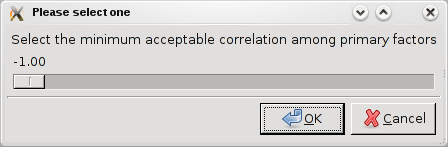
\includegraphics[width=3in]{screenshots2/EFA/lower}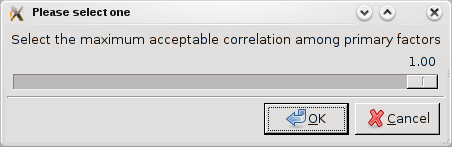
\includegraphics[width=3in]{screenshots2/EFA/upper}\\
The function that imposes this constraint returns $-1$ if $\underline{\Phi}\leq\Phi_{pq}\leq\overline{\Phi}\,\forall p>q$
and otherwise returns the distance between the relevant bound the
the correlation that most egregiously fails to satisfy these bounds.
\item {}``Positive manifold.'' Similarly, this restriction merely places
a lower bound on $\Upsilon_{jp}\,\forall j,p$. Let $\Upsilon^{\ast}\leq0$
be this lower bound, which can be specified interactively by responding
the to following dialog:%
\footnote{This constraint can be enforced at the command line with \Rcode{Rotate(EFA, criteria = list("positive\_manifold"), methodArgs(pm\_threshold = -0.1))}%
}\\
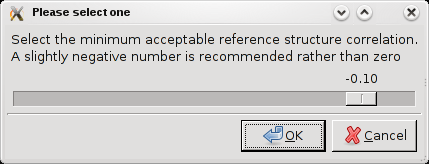
\includegraphics{screenshots2/EFA/pm}\\
The function that imposes this constraint is formally defined as\begin{eqnarray*}
\frac{-1}{nr}\sum_{j=1}^{n}\sum_{p=1}^{r}\mathbb{I}\left\{ \Upsilon_{jp}\geq\Upsilon^{\ast}\right\}  & \in & \left[-1,0\right]\end{eqnarray*}
and hence is satisfied if and only if the proposed $\mathbf{T}$ yields
a {}``positive'' manifold.
\end{itemize}

\subsubsection{The ultimate analytic criterion}

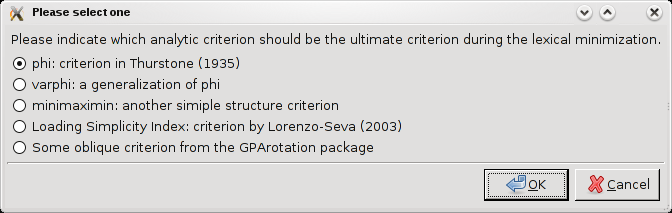
\includegraphics{screenshots2/EFA/criteria1}

The next step is to choose the ultimate criterion for lexical optimization,
as shown in the above dialog box. These criteria are defined as follows:
\begin{itemize}
\item phi: This criterion was proposed by Thurstone (1935) to numerically
characterize simple structure when it reaches its theoretical minimum
of (log) zero. The criterion is formally defined as\begin{eqnarray*}
 & \ln\left(\sum_{j=1}^{n}\exp\left(\frac{1}{c}\sum_{p=1}^{r_{1}}\ln\left(\Upsilon_{jp}^{2}\right)\right)\right),\end{eqnarray*}
which is equal to logarithm of $\phi$ as defined by Thurstone (1935)
when $c=1$. Thurstone suggested that choosing $c$ to be greater
than $1.0$ could yield better results by lessening the pressure to
get one exact zero into each row of $\boldsymbol{\Upsilon}$ and increasing
the pressure to get more than one near-zero into some rows of $\boldsymbol{\Upsilon}$.
If Thurstone's criterion is used, the following dialog box will appear,
prompting the user for $c$:%
\footnote{This pop-up menu can be avoided from the command line with \Rcode{Rotate(EFA, critieria = list("phi"), methodArgs(c = 1))}%
}\\
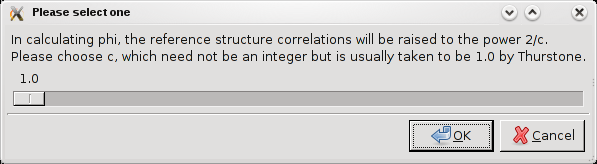
\includegraphics{screenshots2/EFA/c}
\item varphi: This criterion is a generalization of Thurstone's $\phi$.
Let $\overrightarrow{\boldsymbol{\Upsilon}}$ be a matrix of reference
structure correlations where each row is independently sorted in increasing
magnitude, and let $\underset{-\left[1:p\right]}{\overrightarrow{\phi}}$
be Thurstone's criterion (with $c=1$) calculated on $\overrightarrow{\boldsymbol{\Upsilon}}$,
excluding the first through the $p$th column of $\overrightarrow{\boldsymbol{\Upsilon}}$.
Then define $\varphi=\ln\left(\phi+\sum_{p=1}^{r-2}w_{p}\underset{-\left[1:p\right]}{\overrightarrow{\phi}}\right)$,
where $w_{p}\in\left[0,1\right]$ is the weight the analyst specifies
for $\underset{-\left[1:p\right]}{\overrightarrow{\phi}}$ relative
to a unit weight placed on $\phi$. At one extreme, if $w_{p}=0\,\forall p$,
then $\varphi=\phi$. At the other extreme, if $w_{p}=1\,\forall p$,
then the analyst favors a perfect cluster configuration, where three
is only one non-zero coefficient per test. An ``objective'' alternative
to specifying weights is to specify that the weights are a function
of $\overrightarrow{\boldsymbol{\Upsilon}}$, such as $w_{p}=1-\max\left\{ \left(\overrightarrow{\boldsymbol{\Upsilon}}_{p+1}\right)^{2}\right\} ^{\frac{1}{2}}$
to gradually reduce the weight as $p$ increases. These weights can
be specified interactively%
\footnote{These pop-up menus can be avoided from the command line with \Rcode{Rotate(EFA, criteria = list("varphi"), methodArgs(w = rep(0.5, 4))}
to weight all subsequent columns at half th weight of the first, for
example. Or, \Rcode{w} can be any negative number to indicate dynamic
weights.%
}:\\
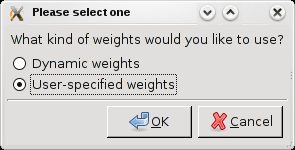
\includegraphics[width=3in]{screenshots2/EFA/weights1}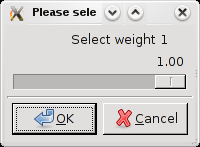
\includegraphics[width=3in]{screenshots2/EFA/weights2}\\

\item minimaximin: This criterion attempts to satisfy Thurstone's definition
of simple structure by choosing $\mathbf{T}$ so that all outcomes
have at least one near-zero reference structure correlation. The criterion
is formally defined as \begin{eqnarray*}
 & \ln\left(\max\left\{ \min\left\{ \Upsilon_{1}^{2}\right\} ,\min\left\{ \Upsilon_{2}^{2}\right\} ,\dots,\min\left\{ \Upsilon_{n}^{2}\right\} \right\} \right).\end{eqnarray*}
Thus, the (log of the) maximum, minimum, squared, row-wise reference
structure correlation is minimized.
\item LS: This criterion is called the Loading Simplicy Index in Lorenzo-Seva
(2003). The derivation of it is not complicated but involves a lot
of notation not previously introduced here, so the reader is refered
to Lorenzo-Seva (2003) for details. Simply put, it reaches its optimum
of (negative) $1.0$ when $\boldsymbol{\Upsilon}$ exhibits a perfect
cluster configuration. Although Lorenzo-Seva (2003) defines the Loading
Simplicity Index in terms of the primary pattern matrix, it is invariant
to the column-scale of the primary pattern matrix and thus can arbitrarily
be defined for the reference structure matrix as well.
\item {}``Some oblique criterion from the GPArotation package.'' If this
option is marked, then the following dialog box appears, unless the
name of the criterion is specified in \Rcode{criteria} in the call
to \Rcode{Rotate}, e.g. \Rcode{Rotate(EFA, criteria = list("quartimin"))}\\
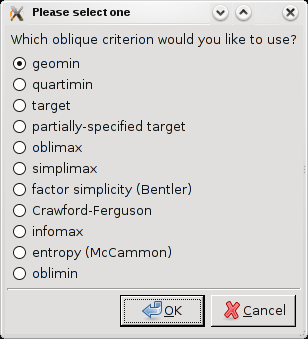
\includegraphics{screenshots2/EFA/criteria2}\\
These criteria are all defined in Browne (2001) and Bernaards and
Jennrich (2006) and documented in the suggested GPArotation package.
The versions in FA$i$R work the same way, with four exceptions. First,
and most importantly, FA$i$R minimizes these criteria subjects to
the aforementioned restrictions. Second, if the criterion has any
additional arguments, they can be specified in a corresponding pop-up
menu (or specified in \Rcode{methodArgs}, as in the GPArotation library).
Third, the partially-specified target implementation allows the partially-specified
target matrix to have \Rcode{NA} in cells that are not targeted,
instead of specifying a separate weight matrix of zeros and ones.
Fourth, in FA$i$R the criteria defined in the GPArotation package
can also be invoked on $\boldsymbol{\Upsilon}$ or $\boldsymbol{\Game}$,
instead of $\boldsymbol{\beta}$ by specifying \Rcode{matrix = "RS"}
or \Rcode{matrix = "FC"} as an element of \Rcode{methodArgs} or
by responding to this dialog:\\
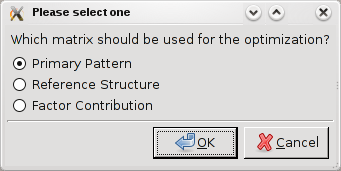
\includegraphics{screenshots2/EFA/matrix}
\end{itemize}

\section{References}

{\small Anderson, T.W. and H. Rubin. 1956. {}``Statistical inference
in factor analysis'' in }\emph{\small Proceedings of the Third Berkeley
Symposium on Mathematical Statistics and Probability}{\small . vol.~5.~no.
1.~University of California Press.}{\small \par}

{\small Bentler, P.M. and P. Dudgeon. 1996. {}``COVARIANCE STRUCTURE
ANALYSIS: Statistical Practice, Theory, and Directions.'' }\emph{\small Annual
Reviews in Psychology}{\small . 47(1):563 -- 592.}{\small \par}

{\small Bernaards, C.A. and R.I.~Jennrich. 2006. {}``Gradient Projection
Algorithms and Software for Arbitrary Rotation Criteria in Factor
Analysis.'' }\emph{\small Educational and Psychological Measurement}{\small .
65(5):676 -- 696.}{\small \par}

{\small Bollen, K.A.~and K.G. J\"{o}reskog. 1985. {}``Uniqueness
does not Imply Identification: A Note on Confirmatory Factor Analysis.''
}\emph{\small Sociological Methods and Research}{\small . 14(2):155
-- 163.}{\small \par}

{\small Browne, M.W. 2001. {}``An Overview of Analytic Rotation in
Exploratory Factor Analysis.'' }\emph{\small Multivariate Behavioral
Research}{\small . 36(1):111 -- 150.}{\small \par}

{\small Butler, J.M. 1969. ``Simple Structure Reconsidered: Distinguishability
and Invariance in Factor Analysis.'' }\emph{\small Multivariate Behavioral
Research}{\small{} 4(1):5 \textendash{}- 28.}{\small \par}

{\small Conger, J.A. 1974. {}``A Revised Definition for Suppressor
Variables: a Guide To Their Identification and Interpretation.''
}\emph{\small Educational and Psychological Measurement}{\small .
34(1):35 -- 46}{\small \par}

{\small Dey, D. K.~and K.~Srinivasan. 1985. {}``Estimation of a
covariance matrix under Stein's loss.'' }\emph{\small The Annals
of Statistics}{\small . 13:1581 -- 1591.}{\small \par}

{\small Goodrich, B. 2008a. ``SEFA$i$R So Far.'' Unpublished manuscript
available from the FA$i$R wiki \url{http://wiki.r-project.org/rwiki/doku.php?id=packages:cran:fair}}{\small \par}

{\small Goodrich, B. 2008b. ``Restrictions, Factor Analysis, and Genetic
Algorithms.'' Unpublished manuscript available from the FA$i$R wiki
\url{http://wiki.r-project.org/rwiki/doku.php?id=packages:cran:fair}}{\small \par}

{\small Harman, H.H. 1976. }\emph{\small Modern Factor Analysis}{\small .
University Of Chicago Press.}{\small \par}

{\small Howe, W.G. 1955. Some Contributions to Factor Analysis. Technical
report ORNL-1919, Oak Ridge National Lab., Tenn.}{\small \par}

{\small Koopmans, T.C. and O. Reiers\o{}l. 1950. {}``The identification
of structural characteristics.'' }\emph{\small Annals of Mathematical
Statistics}{\small . 21(1):165 -- 181.}{\small \par}

{\small Lorenzo-Seva, U. 2003. \textquotedblleft{}A factor simplicity
index.\textquotedblright{} }\emph{\small Psychometrika}{\small{} 68(1):49
-- 60.}{\small \par}

{\small Millsap, R.E. 2001, {}``When Trivial Constraints Are Not
Trivial: The Choice of Uniqueness Constraints in Confirmatory Factor
Analysis.'' }\emph{\small Structural Equation Modeling}{\small .
8(1):1 -- 17.}{\small \par}

{\small Opgen-Rhein, R., and K. Strimmer. 2007. {}``Accurate ranking
of differentially expressed genes by a distribution-free shrinkage
approach.'' }\emph{\small Statistical Applications in Genetics and
Molecular Biology}{\small . 6(1), article 9.}{\small \par}

{\small Pe\~{n}a, D. and J. Rodr\'{i}guez. 2003. ``Descriptive measures
of multivariate scatter and linear dependence.'' }\emph{\small Journal
of Multivariate Analysis}{\small{} 85(2):361 -- 374.}{\small \par}

{\small Pison, G., Van Aelst, S., and Willems, G. 2002. {}``Small
Sample Corrections for LTS and MCD.'' }\emph{\small Metrika}{\small .
55:111 -- 123.}{\small \par}

{\small Reiers\o{}l, O. 1950. {}``On the Identifiability of Parameters
in Thurstone's Multiple Factor Analysis.'' }\emph{\small Psychometrika}{\small .
15:121 -- 149.}{\small \par}

{\small Rousseeuw, P.J. and K.~Van Driessen. 1999. {}``A fast algorithm
for the minimum covariance determinant estimator.'' Technometrics.
41(3):212 -- 223.}{\small \par}

{\small Schä\"{a}fer, J., and K. Strimmer. 2005. {}``A shrinkage
approach to large-scale covariance matrix estimation and implications
for functional genomics.'' }\emph{\small Statistical Applications
in Genetics and Molecular Biology}{\small . 4(1), article 32.}{\small \par}

{\small Thurstone, L.L. 1935. }\emph{\small The vectors of mind: multiple-factor
analysis for the isolation of primary traits}{\small . University
of Chicago Press.}{\small \par}

{\small White, O. 1966. {}``Some Properties Of Three Factor Contribution
Matrices.'' }\emph{\small Multivariate Behavioral Research}{\small .
1(3):373 -- 377.}{\small \par}

{\small Yates, A. 1987. }\emph{\small Multivariate exploratory data
analysis: A perspective on exploratory factor analysis}{\small . State
University of New York Press.}
\end{document}
